\documentclass{sig-alternate}
%\documentclass{acm_proc_article-sp}
%\documentclass[times, 10pt,twocolumn]{article} 
\pagestyle{empty}
%\usepackage{latex8}
\usepackage{times}
\usepackage{algorithm}
\usepackage{algorithmic}

%\usepackage{algorithm2e}

\usepackage{graphicx}
\usepackage{epsfig}
\usepackage{url}
\input{macros}

\begin{document}
\title{eXpress: Guided Path Exploration for Regression Test Generation}

\author{
Kunal Taneja$^1$, \hspace{0.05in} Tao Xie$^1$,  \hspace{0.05in} Nikolai Tillmann$^2$,  \hspace{0.05in} Jonathan de Halleux$^2$,   \hspace{0.05in} Wolfram Schulte$^2$\\
       \small{$^1$Department of Computer Science, North Carolina State University, Raleigh, NC, 27695, USA}\\
       \small{$^2$Microsoft Research, One Microsoft Way, Redmond, WA, 98074, USA}\\
       \small{$^1$\{ktaneja, txie\}@ncsu.edu, $^2$\{nikolait, jhalleux, schulte\}@microsoft.com} 
}   
%\vspace{-0.6 in}
\maketitle
\thispagestyle{empty}

\begin{abstract}
Code Search Engines (CSE) can serve as powerful resources of open
source code, as they can search in billions of lines of open source
code available on the web. The strength of CSEs can be used for
several tasks like searching relevant code samples, identifying
hotspots, and finding bugs. However, the major limitations in using
CSEs for these tasks are that the returned samples are too many and
they are often partial. Our framework addresses the preceding
limitations and thereby helps in using CSEs for these tasks. We
showed the effectiveness of our framework with two tools developed
based on our framework.

\Comment{CSEs are often used by programmers to search for relevant
code samples from publicly accessible source code. However, CSEs are not quite
helpful in practice because the number of returned samples are too many and
the desired code sample is often not available among the first several results.
Apart from using CSEs for searching relevant code samples, CSEs can also be used
for several other applications like identifying framework hotspots and finding bugs
in software. Exploiting CSEs for these applications requires analysis of
the code samples returned by CSEs. This analysis is non-trivial because the code samples
returned by CSEs are often partial.\Comment{, as CSEs retrieve
only source files with usages of the given query instead of entire projects.}
In this paper, we propose an extensible framework that addresses the preceding limitations
and thereby helps in exploiting CSEs for several applications that can help improve the
productivity of programmers. Our framework performs static analysis over code samples gathered from a CSE by
using several heuristics and transforms those samples into graph representations that can be directly
used for other applications. }
\end{abstract}


\section{Introduction}
\label{Introduction}

In software testing, test-adequacy criteria play an important role
in determining whether the software under test (SUT) is adequately
tested~\cite{Goodenough:75,Zhu:96}. With a test-adequacy criterion,
a tester can continually create new test cases until the suite of
test cases created so far satisfies the criterion. $Mutation$
$testing$, which was first proposed by Hamlet~\cite{Hamlet:77} and
DeMillo et al.~\cite{DeMillo:78}, is an intensively studied way to
construct such a test-adequacy criterion. In mutation testing, many
faulty versions (known as $mutants$) of the SUT are generated
through automatically changing the SUT with $mutation$ $operators$,
each of which is a rule to produce faulty versions and can be
applied to various statements. Since the first proposal, mutation
testing has attracted the attention of many researchers (e.g., Acree
et al.~\cite{Acree:79}, Budd et al.~\cite{Budd:80b}, Wong and
Mathur~\cite{Mathur:91,Wong:93,Wong:95}, Offutt et
al.~\cite{Offutt:92,Offutt:94,Offutt:96,Offutt:97,Offutt:99,Ma:05},
Mresa et al.~\cite{Mresa:99}, Hierons and Harman~\cite{Hierons:99},
Barbosa et al.~\cite{Barbosa:01}, and Zeller et
al.~\cite{Grun:09,Schuler:09}). Recently, researchers used mutation
operators to automatically produce faulty software to facilitate
experimentation in research of software
testing~\cite{Briand:04,Briand:06,Mayer:06,Tuya:07}. Andrews et
al.~\cite{Andrews:05} and Do et al.~\cite{Do:06} reported some
evidence that faults generated with mutation operators are similar
to real faults in evaluating test effectiveness. Following the
terminology of Andrews et al.~\cite{Andrews:05,SiamiNamin:08}, we
refer to this way of using mutation as $mutation$ $analysis$.

Mutation testing and mutation analysis are usually very
expensive~\cite{Budd:80b,Mathur:91,Wong:93,Offutt:96,SiamiNamin:08}.
For example, Proteum~\cite{Delamaro:96} generates 4,937 mutants for
$tcas$ (which is the smallest program among the Siemens
programs~\cite{Hutchins:94} and contains only 137 non-commenting and
non-whitespace lines of code) using 108 mutation operators. Thus,
compiling and executing a large number of mutants can be a big
burden in mutation testing and analysis. To alleviate this burden,
researchers have proposed various
techniques~\cite{Acree:79,Mathur:91,Wong:93,Wong:95,Offutt:96,Barbosa:01,SiamiNamin:08}
for selecting a subset of all the mutants. Naturally, researchers
want the set of selected mutants to be similar to the set of all
mutants. One simple technique is random mutant
selection~\cite{Acree:79,Wong:93,Wong:95}, in which, given a fixed
percentage number (denoted as $x$), $x\%$ mutants are randomly
selected. However, researchers seem to be more enthusiastic at
investigating operator-based mutant
selection~\cite{Mathur:91,Wong:93,Wong:95,Offutt:96,Barbosa:01,SiamiNamin:08},
which aims to select mutants generated with only a set of sufficient
mutation operators\footnote{A set of mutation operators are
sufficient if the mutants generated by the mutation operators can
very much represent the mutants generated by all the mutation
operators.}. While early research on operator-based mutant
selection~\cite{Wong:93,Wong:95,Offutt:96} tries to determine
sufficient mutation operators via simple rules, recent
research~\cite{Barbosa:01,SiamiNamin:08} relies on sophisticated
procedures to determine sufficient mutation operators involving
statistical information that can be acquired only through executing
a large number of mutants with a sufficiently large set of test
cases.

Despite the enthusiasm in investigating operator-based mutant
selection, whether operator-based mutant selection is superior to
random mutant selection for mutation testing remains an open
question. That is to say, despite recent progress in operator-based
mutant selection (e.g., Offutt et al.~\cite{Offutt:96}, Barbosa et
al.~\cite{Barbosa:01}, and Siami Namin et al.~\cite{SiamiNamin:08}),
there is lack of empirical evaluation of these operator-based
mutant-selection techniques against random mutant selection
techniques. Furthermore, as we can view random mutant selection as
an approach to mutant selection with average effectiveness,
answering the preceding open question can help us gain insights and
deep understanding to the current research and achievements on
mutant selection.

In this paper, we report an empirical study attempting to answer
this open question. To evaluate the effectiveness of each
mutant-selection technique, we adopt a widely used metric for
evaluating mutant-selection techniques. The metric aims to measure
to what extent the selected mutants are able to represent the
whole set of mutants. Furthermore, we also evaluate the stability
of each technique by checking how consistently the technique
performs under different circumstances. For either effectiveness
or stability, our empirical results do not support that
operator-based mutant selection is superior to random mutant
selection. That is to say, random mutant selection remains a
competitive or even better choice compared with recent progress in
operator-based mutant selection. Furthermore, as random mutant
selection selects mutants on the basis of individual mutants
instead of mutation operators, our empirical results also indicate
that mutant-selection techniques based on individual mutants
should be worthy of further investigation.

The main contributions of our study are as follows.


\begin{itemize}
\vspace{-2ex}

\item Our study empirically evaluates three recent operator-based
mutant-selection techniques (i.e., Offutt et al.~\cite{Offutt:96},
Barbosa et al.~\cite{Barbosa:01}, and Siami Namin et
al.~\cite{SiamiNamin:08}) against random mutant selection for
mutation testing.\vspace{-2ex}

\item Our study produces the first empirical results concerning
stability of operator-based mutant selection and random mutant
selection for mutation testing. \vspace{-2ex}

\item Beside the random technique studied previously (referred to as
the one-round random technique in this paper), our study also
investigates another random technique involving two steps to select
each mutant (referred to as the two-round random technique in this
paper).\vspace{-2ex}

\item The subjects used in our study are larger than those used in
previous studies of random mutant selection. To the best of our
knowledge, due to the extreme expensiveness of experimenting
mutant-selection techniques, the Siemens programs are by far the
largest subjects\footnote{Some studies on mutation testing and
analysis (such as Do et al.~\cite{Do:06}) do use larger subjects,
but they do not focus on mutant selection and they do not consider
all the generated mutants.} used in studies of mutant
selection~\cite{SiamiNamin:08}. \vspace{-2ex}

\end{itemize}

We organize the rest of this paper as follows.
Section~\ref{Experiment} presents the experimental design in our
study. Section~\ref{Results} presents and analyzes the results
obtained from our experiments. Section~\ref{Discussion} discusses
other issues in our study. Section~\ref{RelatedWork} discusses
related work. Section~\ref{Conclusion} concludes and presents some
future work.

\section{Rule Templates}
\label{sec:ruletmpl}

\begin{figure}[t]
\begin{CodeOut}
\begin{alltt}
01:public static void verifyBCEL(String cName) \{ 
02:\hspace*{0.1in}VerificationResult vr0, vr1, vr2, vr3; 
03:\hspace*{0.1in}int mId = 0;
04:\hspace*{0.1in}Verifier verf = VerifierFactory.getVerifier(cName);
05:\hspace*{0.1in}if(verf != null) \{ 	
06:\hspace*{0.2in}vr0 = verf.doPass1();
07:\hspace*{0.2in}if(vr0 != VerificationResult.VR\_OK)
08:\hspace*{0.4in}return;
09:\hspace*{0.2in}vr1 = verf.doPass2();	
10:\hspace*{0.2in}if (vr1 == VerificationResult.VR\_OK) \{ 
11:\hspace*{0.4in}JavaClass jc = Repository.lookupClass(cName);
12:\hspace*{0.4in}for(mId=0; mId<jc.getMethods().length; mId++)\{ 
13:\hspace*{0.5in}vr2 = verf.doPass3a(mId);
14:\hspace*{0.5in}vr3 = verf.doPass3b(mId);
15:\hspace*{0.5in}if(Pass3aVerifier.do\_verify(verf)) \{ ... \}
16:\hspace*{0.1in}\} \hspace*{0.2in}\} \hspace*{0.1in}\} \} 
\end{alltt}
\end{CodeOut}\vspace{-5ex}
\Caption{\label{fig:patternex} Code sample gathered from a code search engine.}\vspace{-4ex}
\end{figure}

We next present the rule templates defined by our approach for
capturing programming rules around individual API calls (for generality,
we refer methods in an API as individual API calls). We use the code example
shown in Figure~\ref{fig:patternex} as an illustrative example for
describing our rule templates. 

In general, a method invocation
in Java consists of four elements: the receiver object, method name, arguments, and return object.
For example, the method invocation in Statement 13 of the code example has the receiver object \CodeIn{verf},
argument \CodeIn{mId}, and the return object \CodeIn{vr2}.
The condition checks for a method invocation can appear before the call site (say, preceding conditions),
or can appear after the call site (say, succeeding conditions). More specifically,
we are interested in condition checks on the receiver object and arguments 
before a call site and condition checks on the receiver object and return object after
the call site. To capture such condition checks as programming rules, 
we define a rule template and a programming rule as follows:\\

\textbf{Definition 1:} \emph{A rule template is a five-tuple ($T_{type}$, $O_{type}$, $MI$, $AI$, $POS$), where\\
\hspace*{0.3in}$T_{type}$: template type\\
\hspace*{0.3in}$O_{type}$: object type such as a receiver or return\\
\hspace*{0.3in}$MI$: method invocation\\
\hspace*{0.3in}$AI$: optional additional information\\
\hspace*{0.3in}$POS$: location with respect to a call site}

\textbf{Definition 2:} \emph{A programming rule is an instance of a rule template.}\\

The element $T_{type}$ (template type) of a rule template describes
the type of the condition checks in the programming rule, whereas the element $O_{type}$ (object type)
represents the participating object of the individual API call such as the receiver,
argument, or return object. The element $MI$ (method invocation) stores the individual API call.
The element $AI$ is optional additional information associated with each programming
rule. The information stored in the $AI$ element is dependent on $T_{type}$.
As we capture both preceding and succeeding programming rules, the element
$POS$ describes the location of the programming rule with respect to the call site of an 
individual API call. We next describe each element in detail.

\setlength{\tabcolsep}{1pt}
\begin{table*}[t]
\begin{SmallOut}
\begin{CodeOut}
\begin{center}
\centering \caption {\label{tab:conditiontypes} Possible $T_{type}$ values of a rule template and associated
additional information}
\begin {tabular} {|l|l|l|c|}
\hline
Name&\CenterCell{Description}&\CenterCell{Additional Info}&\CenterCell{Coverage}\\
\hline
\hline direct-null-check&direct null check. e.g., if(var != null) \{ .. \}&operator involved, e.g., != & 97/497\\
\hline indirect-null-check&if variable is an argument of a &operator involved, e.g., == & 2/497 \\
		   &method invocation. e.g., if(MI(var) == null) \{ .. \}&method invocation, MI&\\
\hline direct-boolean-check&if the variable type is boolean. e.g., if(var) \{ .. \}& &65/497\\
\hline indirect-boolean-check&indirect boolean check. e.g., if(MI(var)) \{ .. \}&method invocation, e.g., MI& 25/497\\
\hline direct-const-check&if the variable is compared with a constant.&operator involved, e.g., ==&110/497\\
			 & e.g., if(var == SUCCESS)&constant value, e.g., SUCCESS&\\
\hline indirect-const-check&indirect constant equality check.&operator involved, e.g., ==&1/497\\
		 	 & e.g., if(MI(var) == FAILURE)&constant value, e.g., FAILURE&\\
		 	 & &method invocation, e.g., MI&\\
\hline direct-retval-check&if the variable is compared with the&operator involved, e.g., <&0/497\\
			 &return value of a method invocation.&method invocation, e.g., $MI_{other}()$&\\
			 &e.g., if(var < $MI_{other}()$)&&\\ 
\hline indirect-retval-check&if the variable is compared indirectly with the&operator involved, e.g., >&0/497\\
			 &return value of a method invocation.&method invocation, e.g., MI&\\
			 &e.g., if(MI(var) > $MI_{other}()$)&method invocation, e.g., $MI_{other}()$&\\ 
\hline instance-check&if the conditional check involves \CodeIn{instanceof} operator&type-name, e.g., Integer&106/497\\
			 &e.g., if(var instanceof Integer)&&\\
\hline direct-expr-check&if the variable is compared with an &operator involved, e.g., <&35/497\\
			 &expression such as another variable. e.g., if(var < expr) \{ ... \}&other expression, e.g., expr&\\		 			 			 
\hline
\end{tabular}
\end{center}
\end{CodeOut}
\end{SmallOut}
\vspace*{-4ex}
\end{table*}

Table~\ref{tab:conditiontypes} shows several possible values for the $T_{type}$ element
of the rule template. For each template type, we present the name, description with an example, 
and additional information ($AI$) that is associated with the programming rule. 
The additional information is dependent on the $T_{type}$ element.
For example, the template type \CodeIn{direct-null-check} 
captures programming rules such as \CodeIn{null} checks done on the receiver, arguments, or return objects. 
In the description of each template type, we use notation \CodeIn{var} 
to denote a receiver, argument, or return object of the individual API call. The additional
information for the template type \CodeIn{direct-null-check} stores the operator involved in the 
conditional expression such as ``=='' or ``!=''. Column ``Coverage'' shows the number
of rules that belong to each template type divided by the total number of 
rules that we found in our preliminary investigation with BCEL. All template
types described in the table include 88\% of the rules we found during our investigation.

Our template types are broadly classified into two different
categories: direct and indirect. The rationale behind these two categories 
is that a condition check can be performed directly on the variable or
can be done indirectly through another method invocation, say MI, where the current
variable is an argument of that method invocation. The template
type \CodeIn{indirect-null-check} in the table is an example for the indirect template type. 
For indirect template types, the optional additional information 
also stores the associated method invocation. This gathered additional information 
for each programming rule is later used while detecting violations.

Apart from template types shown in the table, we define two more template types
that are specific to the receiver object of a method invocation. 

\textbf{before.} this template type represents condition checks 
on other method invocations of the same receiver object preceding the call site of 
an individual API call. For example, Statements 6 to 9 in the code example
describe that before invoking the \CodeIn{doPass2} method, the method \CodeIn{doPass1} must
be invoked and a condition check must be performed on the return value of the method \CodeIn{doPass1}.
The corresponding programming rule can be captured by this template type as ``\CodeIn{direct-const-check} on \CodeIn{return} of \CodeIn{doPass1} \CodeIn{before} \CodeIn{doPass2}''.

\textbf{after.} this template type captures condition checks on other method invocations
of the same receiver object succeeding the call site of an individual API call. In general, 
this template type is useful for methods such as \CodeIn{Iterator.next()} and 
\CodeIn{Iterator.hasNext()} that are often used in loops, where
one of the methods such as \CodeIn{hasNext} is involved in the conditional expression of the loop. If not,
this template type can result in many false positives based on our
empirical investigation. Therefore, in the NCDetector framework,
we limit this template type to those APIs (such as Java Util APIs) that are often
suggested to be used in loops.

Definition 2 describes programming rules as instances of a rule template. However,
to provide better readability, we present programming rules in a textual form in this paper. 
For example, the programming rule ``\CodeIn{direct-null-check} on \CodeIn{receiver before doPass1}''
indicates that a \CodeIn{null} check should be done on the receiver object of 
\CodeIn{doPass1} before its call site. In this instance, $T_{type}$ is \CodeIn{direct-null-check},
$O_{type}$ is \CodeIn{receiver}, $MI$ is \CodeIn{doPass1}, and $POS$ is \CodeIn{before}.
\section{Example}
\label{sec:example}

\begin{figure*}[t]
\centering
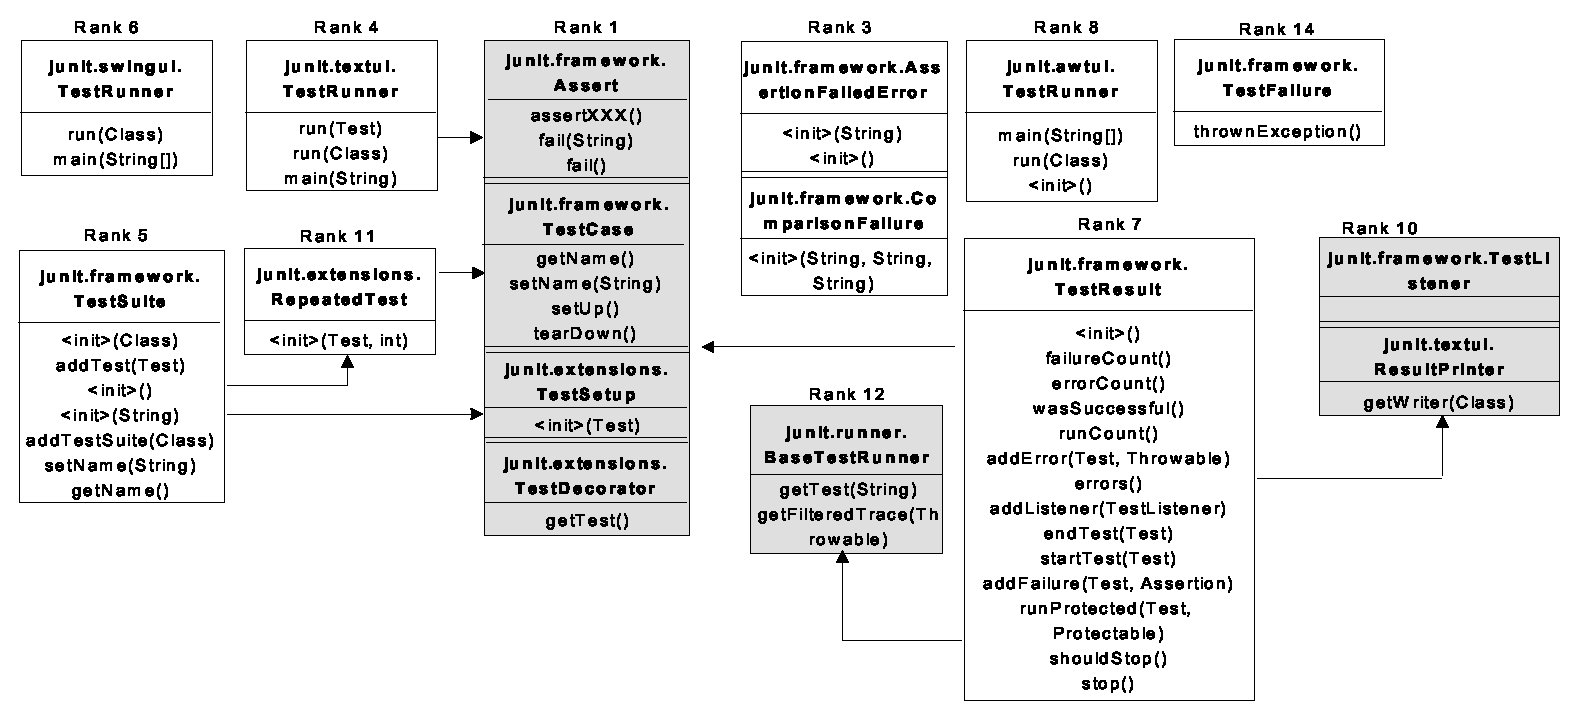
\includegraphics[scale=0.68,clip]{figs/examplehotspot_final.eps}
\caption{Hotspot hierarchies identified for the JUnit framework} \label{fig:hotspotexample}
\end{figure*}

We next use an example to explain our approach and show how the detected
hotspots and coldspots can be used by the framework users. We use JUnit~\cite{JUNIT}, the
\emph{de facto} standard unit testing framework for Java, 
as an illustrative example for explaining our approach.

SpotWeb accepts an input framework, say JUnit, and extracts
\emph{FrameworkInfo} from the framework. The
\emph{FrameworkInfo} includes all classes, all interfaces, public
or protected methods of each class and interface, and inheritance
hierarchy among classes or interfaces of the framework. SpotWeb also captures
the constants defined by the input framework. SpotWeb
constructs different queries for each class or interface and
interacts with a CSE such as Google code search~\cite{GCSE} to
gather relevant code examples from existing open source projects that
reuse the classes of the input framework. For example, SpotWeb constructs
a query such as ``\CodeIn{lang:java junit.framework.TestSuite}'' for
gathering relevant code examples of the \CodeIn{TestSuite} class. These
gathered code examples are referred as a \emph{LocalRepository} for
the input framework. SpotWeb analyzes gathered code examples
statically and computes \emph{UsageMetrics} for classes, interfaces,
and public or protected methods of all classes and interfaces. For
example, the \emph{UsageMetrics} computed for the \CodeIn{TestSuite}
class show that the class is instantiated for 165 times and is
extended for 32 times. Similarly, the \emph{UsageMetrics} computed
for the method \CodeIn{addTest} of the \CodeIn{TestSuite} class show
that the method is invoked for 95 times. SpotWeb also gathers code
examples for each class or method and stores these code examples in
a repository, referred as \emph{ExampleDB}. Then SpotWeb uses the
algorithm shown in Figure~\ref{alg:hotspotalgo} for detecting
hotspots from the computed \emph{UsageMetrics}.

Initially, SpotWeb ranks methods in a non-ascending order based on
their \emph{UsageMetrics} and uses a threshold percentage $HT$ to
detect hotspot methods: the methods in the top $HT$ percentage with
a non-zero \emph{UsageMetrics} are detected as hotspot methods. 
The detected hotspot methods are then
grouped into their declaring classes, detected as hotspot classes.
These hotspot classes are ranked based on the minimum rank of the
hotspot methods declared by these classes. SpotWeb classifies the
hotspot classes into two categories (templates and hooks) based on
heuristics described in Step 4 of the algorithm shown in Figure~\ref{alg:hotspotalgo}. The hotspot classes of each
category are further grouped into hierarchies based on their
inheritance relationships. For example, SpotWeb detected classes
\CodeIn{Assert} and \CodeIn{TestCase} as hook hotspots in the JUnit
framework. As \CodeIn{TestCase} class extends \CodeIn{Assert} class,
SpotWeb groups both the classes into the same hierarchy. SpotWeb
assigns a rank to each hierarchy based on the minimum rank of the
hotspot classes contained in the hierarchy. For example, consider
that the \CodeIn{Assert} class has Rank 1 and the \CodeIn{TestCase}
class has Rank 2, then the grouped hierarchy of the
\CodeIn{Assert} and \CodeIn{TestCase} classes is assigned with Rank
1. The rank attribute uniquely identifies a hierarchy among all
other hierarchies. Hierarchies with smaller ranks have higher preference
or importance to the hierarchies with larger ranks.

Figure~\ref{fig:hotspotexample} shows the hotspot hierarchies detected for the JUnit
framework. The figure also shows ranks assigned to each hierarchy.
As the rank attribute uniquely identifies a hierarchy, we use the
rank as an identity for describing a hierarchy.
Each hierarchy includes one or more hotspot classes and is shown as pairs of class and its methods.
For example, Hierarchy 1 (hierarchy with Rank 1) has classes \CodeIn{Assert}, \CodeIn{TestCase}, \CodeIn{TestSetup},
and \CodeIn{TestDecorator}. We show template hierarchies in white and hook hierarchies in gray.
For example, Hierarchy 1 is a hook hierarchy and Hierarchy 3 is a template hierarchy.

Methods inside each class of a hierarchy are sorted
based on their computed \emph{UsageMetrics}. Sorting methods of a class
can assist the framework users in quickly identifying the methods that are often
used inside a given hotspot class. For example, consider the \CodeIn{TestSuite} class
shown in Hierarchy 5. The \CodeIn{TestSuite} class has three constructors \CodeIn{<init>(Class)},
\CodeIn{<init>()}, and \CodeIn{<init>(String)}. However, the \CodeIn{<init>(Class)} constructor
is often used compared to the other two constructors. Due to space limit,
we show all assertion methods such as \CodeIn{assertEquals} and \CodeIn{assertTrue}
of the class \CodeIn{Assert} of Hierarchy 1 as \CodeIn{assertXXX}.

The figure also displays dependencies among hotspot hierarchies
(shown as arrows between hierarchies). SpotWeb captures the
usage relationships among hotspot classes through dependencies.
For example, Hierarchy $5$ has a
\CodeIn{TEMPLATE\_HOOK} dependency with Hierarchy $1$. This
dependency indicates that to reuse methods such as \CodeIn{addTest}
of the class \CodeIn{TestSuite} in Hierarchy 5, the user has to
define a new behavior for the classes in Hierarchy $1$.

\begin{figure}[t]
\begin{CodeOut}
\begin{alltt}
01:public class SRDAOTestCase 
02:\hspace*{0.4in}extends TestCase \{
03:\hspace*{0.1in}private SRDAO dao = null;...
04:\hspace*{0.1in}public SRDAOTestCase() \{
05:\hspace*{0.3in}super(); ... 
06:\hspace*{0.1in}\}
07:\hspace*{0.1in}protected void setUp() throws Exception \{
08:\hspace*{0.3in}...
09:\hspace*{0.3in}dao = (SRDAO)context.getBean("SRDAO");
10:\hspace*{0.3in}...
11:\hspace*{0.1in}\}
12:\hspace*{0.1in}public void tearDown() throws Exception \{
13:\hspace*{0.3in}dao = null; 
14:\hspace*{0.1in}\}
15:\hspace*{0.1in}public void testF() \{ ... \}
16:\hspace*{0.1in}public void testB() \{ ... \}
17:\hspace*{0.1in}...
18:\}
\end{alltt}
\end{CodeOut}
\Caption{\label{fig:hcodeexample} Suggested code example for the hook class \CodeIn{TestCase}.}
\begin{CodeOut}
\begin{alltt}
01:public class MyTestSuite \{ 
02:\hspace*{0.1in}...
03:\hspace*{0.1in}public static Test suite() \{
04:\hspace*{0.3in}TestSuite suite = new TestSuite("axis");
05:\hspace*{0.3in}suite.addTest(new SRDAOTestCase());
06:\hspace*{0.3in}return suite;
07:\hspace*{0.1in}\}
08:\hspace*{0.1in}...
09:\}
\end{alltt}
\end{CodeOut}
\Caption{\label{fig:tcodeexample} Suggested code example for the template class \CodeIn{TestSuite}.}
\end{figure}

We next describe how the hotspots detected by SpotWeb can be used by
the framework users to reuse classes of the JUnit framework. After reviewing
the hotspots shown in Figure~\ref{fig:hotspotexample}, consider that
a framework user wants to start with the method \CodeIn{addTest} of
the template class \CodeIn{TestSuite} in Hierarchy 5.
Figure~\ref{fig:hotspotexample} shows that Hierarchy 5 of the
\CodeIn{TestSuite} class has a \CodeIn{TEMPLATE\_HOOK} dependency
with the Hierarchy 1. This dependency indicates that the user may
need to define a new behavior for the associated hook hierarchy.
SpotWeb recommends the code example shown in
Figure~\ref{fig:hcodeexample} for the hook class \CodeIn{TestCase},
which is part of Hierarchy 1. The code example exhibits several
aspects that need to be handled by the user while extending the
\CodeIn{TestCase} class. For example, in the \CodeIn{setUp} method,
the user can write code for setting up the environment such as
instantiating necessary variables, and in the \CodeIn{tearDown}
method, the user can destroy the created variables. In addition, the code
example shows that names of the test methods in the extended class
of the \CodeIn{TestCase} class should start with the prefix \CodeIn{test}.
SpotWeb also recommends a code example for the \CodeIn{addTest} method and
the recommended code example is shown in
Figure~\ref{fig:tcodeexample}. The code example shows that the user
has to create an instance of the \CodeIn{TestSuite} class and then
add test cases through the \CodeIn{addTest} method.

An API class or method is identified as a coldspot if that class or method is neither
used directly nor used indirectly by gathered code examples. The complete
algorithm used for detecting coldspots is shown in Figure~\ref{alg:coldspotalg}. SpotWeb identified $20$
classes such as \CodeIn{Swapper}, \CodeIn{TestRunListener}, and \CodeIn{ExceptionTestCase} as coldspots
in the JUnit framework. However, coldspots are only suggestions
for users unfamiliar to that framework and SpotWeb does not intend to recommend users not to reuse
those coldspot classes. Sometimes, coldspots can also be helpful to
the framework developers in distributing their maintenance efforts, because the framework
developers can give a low preference to the coldspot classes.

\section{Approach}
\label{sec:approach}
\begin{figure}[t]
\centering
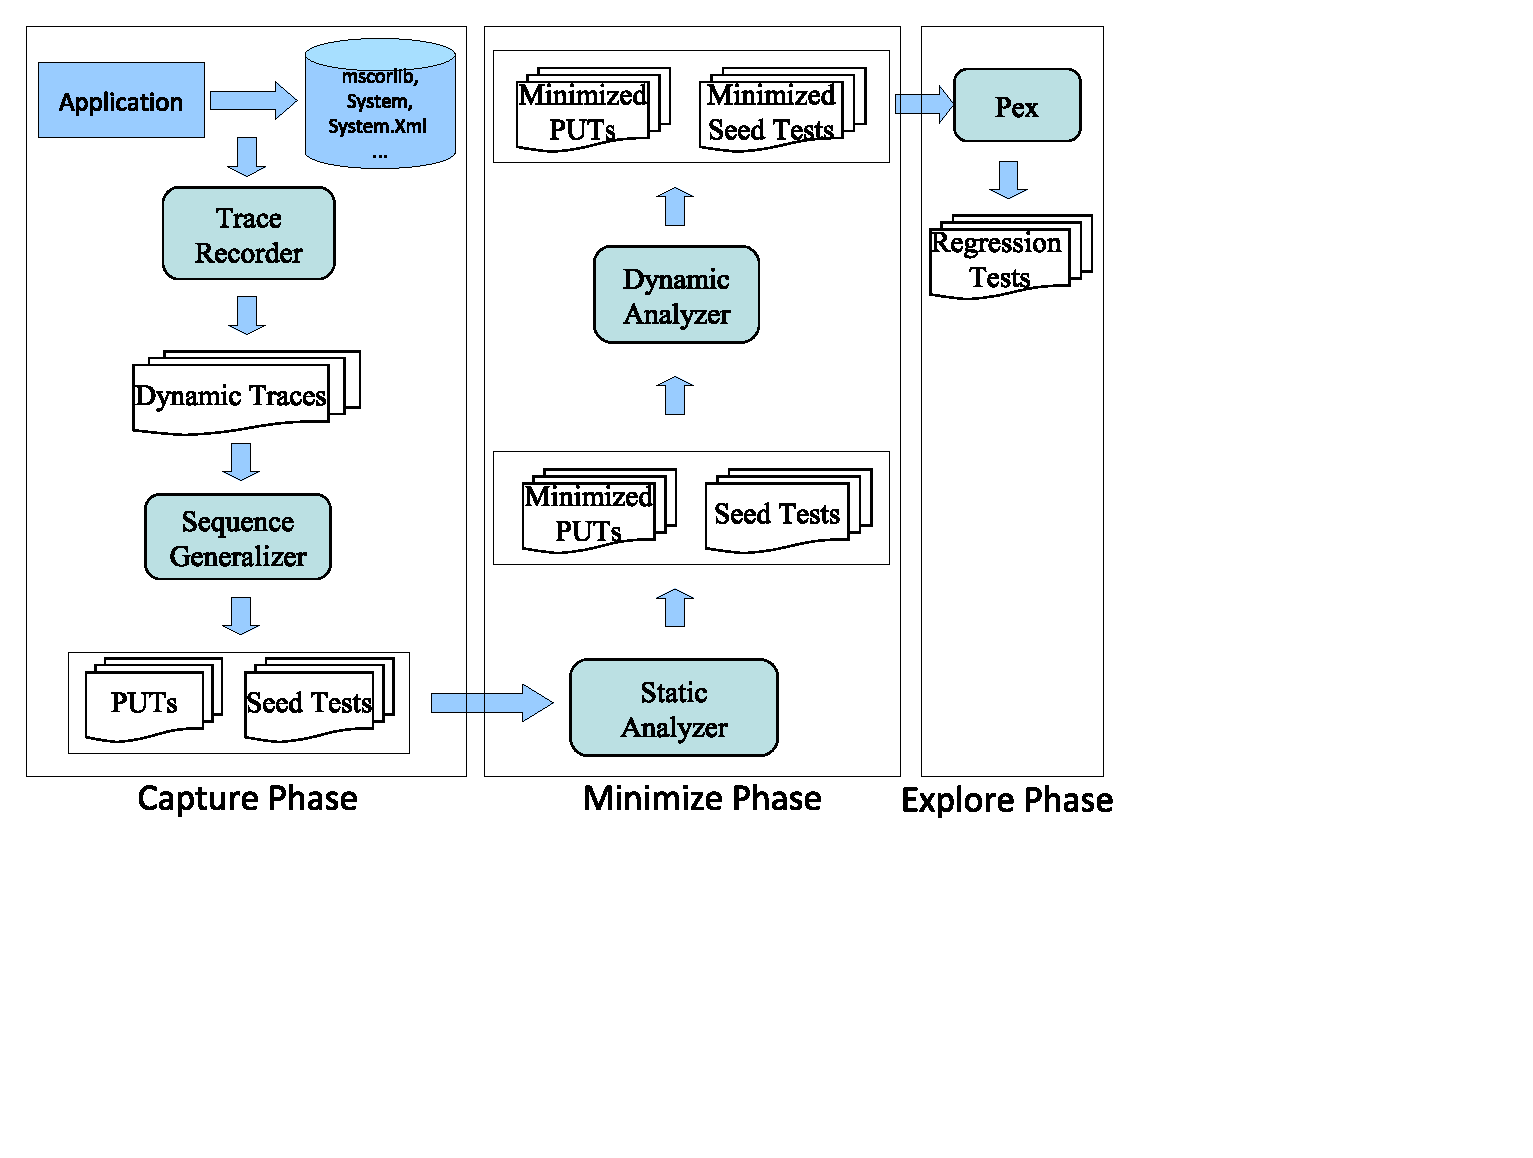
\includegraphics[scale=1,clip]{figure/approach.eps}\vspace*{-3ex}
 \caption{Overview of TeMaAPI}\vspace*{-4ex}
 \label{fig:approach}
\end{figure}
Given a migration tool between Java and C\#, TeMaAPI generates various test cases to reveal different behaviors of the tool's API mapping relations.
Figure~\ref{fig:approach} shows the overview of TeMaAPI.


%-------------------------------------------------------------------
\subsection{Generating client code}
\label{sec:approach:generating}
Given a migration tool, TeMaAPI first extracts its validate mapping relations of APIs. It is challenging to extract such mapping relations directly from a migration tool for two factors: (1) different migration tools may follow different styles to describe API mapping relations. For example, as shown in Section~\ref{sec:introduction}, the API mapping relations of Java2CSharp are described in its mapping files, but the API mapping relations of sharpen are hard-coded in its source files. (2) commercial migration tools typically hide their API mapping relations in binary files. Due to the two factors, TeMaAPI does not extract API mapping relations directly from a migration tool, but chooses to analyze translated code of a migration tool. We choose to use migration tools to translate simple client code instead of existing projects for two considerations: (1) Existing projects typically use quite a small set of APIs, so many API mapping relations may be not covered; (2) a single method of an existing project may use multiple APIs, so it may be difficult to analyze which APIs are not mapped. For the preceding consideration, TeMaAPI chooses to generate client code instead of using existing client code.

TeMaAPI relies on the reflection technique~\cite{maes1987concepts} provided by both Java and C\# to generate client code for translation.

\textbf{Static fields.} Given a public static field \CodeIn{f} of a class \CodeIn{C} whose type is \CodeIn{T}, TeMaAPI generates a getter as follows:
\begin{CodeOut}%\vspace*{-2ex}
\begin{alltt}
 public T TestGet|f.name||no|()\{ return C.f; \}
\end{alltt}
\end{CodeOut}

If \CodeIn{f} is not a constant, TeMaAPI generates a setter as follows:
\begin{CodeOut}%\vspace*{-2ex}
\begin{alltt}
 public void TestSet|f.name||no|(T v)\{ C.f = v; \}
\end{alltt}
\end{CodeOut}

\textbf{Non-static fields.} Given a public non-static field \CodeIn{f} of a class \CodeIn{C} whose type is \CodeIn{T}, TeMaAPI generates a getter for each constructor \CodeIn{C(T1\ p1,\ldots, Tn\ pn)} of \CodeIn{C} as follows:
\begin{CodeOut}%\vspace*{-2ex}
\begin{alltt}
 public T TestGet|f.name||no|(T1\ c1,\ldots, Tn\ cn)\{
    C obj = new C(c1,\ldots, cn);
    return obj.f; \}
\end{alltt}
\end{CodeOut}

If \CodeIn{f} is not a constant, TeMaAPI generates a setter as follows:
\begin{CodeOut}%\vspace*{-2ex}
\begin{alltt}
 public void TestSet|f.name||no|(T1\ c1,\ldots, Tn\ cn)\{
   C obj = new C(c1,\ldots, cn);
   obj.f = v; \}
\end{alltt}
\end{CodeOut}

In the preceding code, ``\CodeIn{|f.name|}'' denotes the name of \CodeIn{f}, and ``\CodeIn{|no|}'' denotes the corresponding number of generated client-code method.

\textbf{Static methods.} Given a public static method \CodeIn{m(T1\ p1,\ldots,Tn\ pn)} of a class \CodeIn{C} whose return type is \CodeIn{Tm}, TeMaAPI generates a client-code method as follows:
\begin{CodeOut}%\vspace*{-2ex}
\begin{alltt}
 public Tm Test|m.name||no|(T1\ m1,\ldots, Tn\ mn)\{
   return C.m(m1,\ldots, mn); \}
\end{alltt}
\end{CodeOut}

\textbf{Non-static methods.} Given a public non-static method \CodeIn{m(T1\ p1,\ldots,Tn\ pn)} of a class \CodeIn{C} whose return type is \CodeIn{Tm}, TeMaAPI generates a client-code method for each constructor \CodeIn{C(Tv\ pv,\ldots, Tt\ pt)} of \CodeIn{C} as follows:
\begin{CodeOut}%\vspace*{-2ex}
\begin{alltt}
 public Tm Test|m.name||no|(T1\ m1,\ldots, Tn\ mn,
                            Tv cv, \ldots, Tt ct)\{
   C obj = new C(cv,\ldots, ct);
   return obj.m(m1,\ldots, mn); \}
\end{alltt}
\end{CodeOut}

In the preceding code, ``\CodeIn{|m.name|}'' denotes the name of \CodeIn{m(T1\ p1,\ldots,Tn\ pn)}.

TeMaAPI ignores generic methods for simplicity, and organizes all generated client code methods by the corresponding class $C$. For a migration tool that translates from Java to C\#, TeMaAPI generates client code in Java as shown by the solid line of Figure~\ref{fig:approach}, and for a migration tool that translates from C\# to Java, TeMaAPI generates client code in C\# as shown by the dotted line of Figure~\ref{fig:approach}. When TeMaAPI generates client code in C\#, it ignores \CodeIn{unsafe} and \CodeIn{delegate} methods and methods whose parameters are marked as \CodeIn{our} or \CodeIn{ref}. Java does not have corresponding keywords, so there are typically no mapped methods in Java for these C\# methods. After TeMaAPI generate client-code methods, we translate them using a migration tool under experiments.


%-----------------------------------------------------------------
\subsection{Analyzing Generated Methods}
\label{sec:approach:analyzing}
Translated code typically contain many compilation errors since a migration tool typically cannot cover mapping relations of all APIs. TeMaAPI then analyzes translated code for validate API mapping relations of the migration tool. To achieve this, TeMaAPI first remove all translated methods with compilation errors. For translated methods in Java, TeMaAPI implements a Eclipse plug-in that uses on Eclipse JDT compiler\footnote{\url{http://www.eclipse.org/jdt/}} for the list of compilation errors. For translated methods in C\#, TeMaAPI implements a Visual Studio.Net add-in to retrieve the list of compilation errors from the error-list view of Visual Studio.Net. Both Eclipse JDT compiler and Visual Studio.Net cannot list all methods with compilation errors in a single build. After each iteration of removing methods, TeMaAPI re-build these methods until it removes all methods with compilation errors.

After methods with compilation errors are removed, TeMaAPI compares generated code with translated code for the validate API mapping relations of a migration tool. Based on translated code and validate API mapping, TeMaAPI removes generated methods whose corresponding translated methods have compilation errors. We refer to those removing client-code methods as safe methods.

%-----------------------------------------------------------
\subsection{Finding Different Behaviors}
\label{sec:approach:behavior}
In the final step, TeMaAPI generates test cases to detect different behaviors of API mapping relations. An alternative approach is to use existing test cases in two languages. For example, lucene\footnote{\url{http://lucene.apache.org}} has both a Java version and a C\# version. It is feasible to use these test cases to reveal some different behaviors, but such test cases typically cover only a small set of APIs. Some test suites such as Java Compatibility Kit (JCK)\footnote{\url{http://jck.dev.java.net}} cover most APIs of a language. However, translating such a test suite from one language into another language may introduce many compilation errors and defects. A test method may use many APIs, so even if the API under test can be translated correctly, the test method cannot be translated correctly since other APIs are not mapped. As a result, we choose to translating existing test suites as a supplement of our approach.

\subsubsection{Generating Test Cases}
\label{sec:approach:behavior:generating}
For each safe method in Java, we use Randoop~\cite{pacheco2007feedback} to generate its test cases. For each safe method in C\#, we use Pex~\cite{tillmann2008pex} to generate its test cases. TeMaAPI then executes generated test cases, and records the inputs, the output, and the thrown exception of each test case as a file.

Based on the file, TeMaAPI generates Junit\footnote{\url{http://www.junit.org/}} or Nunit\footnote{\url{http://www.nunit.org/}} test cases to ensure each mapped API produce the same output give the same inputs. For example, Pex generates a test case whose input is \CodeIn{m0 = false} for the \CodeIn{TestvalueOf57} method in C\# as shown in Section~\ref{sec:example}, and after executing the output of the test case is ``False''. Based on the input and the output of this test case, TeMaAPI generates a Junit test case as follows:

\begin{CodeOut}%\vspace*{-2ex}
\begin{alltt}
 @Test
 public void testvalueOf64zhh0()\{
   sketch.Test_java_lang_String obj =
                       new sketch.Test_java_lang_String();
   boolean m0 = false;
   Assert.assertEquals("False", obj.testvalueOf64(m0));\}
\end{alltt}
\end{CodeOut}

This Junit test case fails since the preceding \CodeIn{testvalueOf64zhh} method produces ``false'' instead of ``False''. From this failed Junit test case, TeMaAPI detects that the \CodeIn{java.lang.String.valueOf (Object)} method in Java has different behaviors with its mapped C\# methods if inputs are boolean values.

In some cases, executing a test case does not produce outputs but exceptions. For example, Pex also generates a test case whose input is \CodeIn{m0 = null} for the \CodeIn{TestvalueOf57} method in C\# as shown in Section~\ref{sec:example}, after executing it throws \CodeIn{NullReferenceException}. TeMaAPI finds that the \CodeIn{NullPointerException} class in C\# is mapped to the \CodeIn{NullPointerException} class in Java in the validate API mapping relations, and generates a Junit test case based on the preceding mapping relation and input as follows:

\begin{CodeOut}%\vspace*{-2ex}
\begin{alltt}
 @Test
 public void testvalueOf64zhh3()\{
   try\{
     sketch.Test_java_lang_String obj =
                       new sketch.Test_java_lang_String();
     boolean m0 = null;
     obj.testvalueOf64(m0);\}
   \}catch(java.lang.NullPointerException e)\{
       Assert.assertTrue(true);
       return;
   \}
   Assert.assertTrue(false);\}
\end{alltt}
\end{CodeOut}

This Junit test case also fails since given a null input, the preceding \CodeIn{testvalueOf64} method does not throw any exceptions. From this failed Junit test case, TeMaAPI detects that the \CodeIn{java.lang. String.valueOf(Object)} method in Java has different behaviors with its mapped C\# methods if inputs are null pointers.

\subsubsection{Translating Existing Test Cases}
\label{sec:approach:behavior:jck}

Each generated client-code method uses only one fields or methods provided by API libraries, and may lose some complicated behaviors even if test cases satisfy the round-trip criterion. To test those complicated behaviors, we introduce JCK that covers many complicated behaviors of Java APIs. JCK is a test suite provided by Sun to ensure compatibility of Java platforms, and it covers most standard APIs of J2SE. However, JCK implements many internal classes to collect the results of executed test cases. If a migration tool cannot correctly translate one of these classes, all translated test cases may have compilation errors or defects. In addition, JCK is released under read-only source license\footnote{\url{http://tinyurl.com/33x9fo6}}, so many such internal classes are not shipped and it has many compilation errors. To increase the chance of migrating JCK, TeMaAPI first replaces those internal classes with the classes of Junit. For example, one test method for \CodeIn{java.io.File.delete()} in JCK is as follows:

\begin{CodeOut}%\vspace*{-2ex}
\begin{alltt}
  public Status File0037()\{
    String testCaseID = "File0037";
    ...
    FileRT method = new FileRT(testCaseID) \{
     public Status run() \{
       File f = null;
       f = new File(workdir, testCaseID);
       ...
       if (f.delete()) \{ // Try to delete
         if (!f.exists()) \{ // Does it exist?
           return Status.passed("OKAY");
         \}else\{
            return Status.failed(...);
         \}
       else\{
           return Status.failed(...);
       \}
    \}
     return AllPermissionSM.testRun(...);
  \}
\end{alltt}
\end{CodeOut}

After the preceding three steps, TeMaAPI further replaces the statement starts with \CodeIn{FileRT} with the body of the \CodeIn{run} method, and removes the last statement. The translated code is as follows:

\begin{CodeOut}%\vspace*{-2ex}
\begin{alltt}
  public void File0037()\{
    String testCaseID = "File0037";
    ...
    File f = null;
    f = new File(workdir, testCaseID);
    ...
    if (f.delete()) \{ // Try to delete
      if (!f.exists()) \{ // Does it exist?
        Assert.assertTrue(true);
        return;
     \}else\{
        Assert.fail();
        return;
     \}
   else\{
       Assert.fail();
       return;
   \}
  \}
\end{alltt}
\end{CodeOut}

Compared with the original test method in JCK, the translated method does not use the three internal classes: \CodeIn{Status}, \CodeIn{FileRT}, and \CodeIn{AllPermissionSM}. 

After the preceding process, for a migration tool, TeMaAPI further removes methods that use any APIs outside its defined mapping relations. The remaining methods can be translated from Java to other languages since it does not use any APIs outside of the migration tool.



\section{Implementation}
\label{sec:implementation}

TODO: Mention here that some of the components from the earlier
paper ASE07 are reused like CodeDownloader, CodeAnalyzer. Also mention
that the previous CodeAnalyzer just analyzes only those statements
that transform one object type to another. Now it has been extended
to handle many other kinds of statements in the Java programming language.
\section{Experiments}
\label{sec:evaluation}

We conducted experiments on four programs and their 72 versions (in total) collected from three different sources. In our experiments, we try to address the following research questions:
%\begin{itemize}
\Comment{
\\ \textbf{RQ1.} How much fewer DSE runs does Pex require to execute the changed regions between the two versions of a program with the assistance of \CodeIn{eXpress}?
	\\ \textbf{RQ2.} Can \CodeIn{eXpress} more efficiently infect the program states after the execution of changed regions than without using \CodeIn{eXpress}?	
	\\ \textbf{RQ3.} Can \CodeIn{eXpress} effectively help generate tests that execute changed regions between the two versions of a program than without using \CodeIn{eXpress}?
	\\ \textbf{RQ4.} Can \CodeIn{eXpress} effectively help generate tests that infect the program states after the execution of changed regions than without using \CodeIn{eXpress}?
	\\ \textbf{RQ5.} Can our approach of seeding the exploration with existing unit-tests efficiently help covering the changed regions and infect program states?
}
\\ \textbf{RQ1.} How much fewer DSE runs does Pex require to execute the changed regions between the two versions of a program with the assistance of \CodeIn{eXpress}?
	\\ \textbf{RQ2.} How much fewer DSE runs does Pex require to infect the program states with the assistance of \CodeIn{eXpress}?
	\\ \textbf{RQ3.} How much more tests does Pex, with the assistance of \CodeIn{eXpress}, generate that execute changed regions between the two versions of a program?
	\\ \textbf{RQ4.} How much more tests does Pex, with the assistance of \CodeIn{eXpress}, generate that infect the program states?
	\\ \textbf{RQ5.} How much fewer DSE runs does Pex require to cover the changed regions when the program exploation is seeded with the existing test suite?

		\Comment{
	\\ \textbf{RQ6.} Can the optimizations used in \CodeIn{Graph Builder} and \CodeIn{Graph Traverser} components of \CodeIn{eXpress} efficiently reduce the time to find irrelevant branches that cannot help in satisfying E of the PIE model?
	

	\item \textbf{RQ3.} Can \CodeIn{eXpress} more efficiently propagate the program state infection to some observable output?
	
	}	
%\end{itemize}

\Comment{
\begin{table*}
\begin{CodeOut}
\begin{center}
\caption {\label{table:siena_results}Experimental Results for Siena}
\begin {tabular} {|l|c|c|c|c|c|c|c|c|}
\hline
\multicolumn{4}{|c|}{}&\multicolumn{2}{|c|}{Reused}&\multicolumn{2}{|c|}{TUT 2 PUT}\\ 
\hline
MUMs&\CenterCell{Methods Implemented
} &\CenterCell{Methods Reused
}&\CenterCell{    Increase in LOC
}&\CenterCell{   Increase in Max. CC  
}&\CenterCell{  Increase in LOC
}&\CenterCell{   Increase in Max. CC
}&\CenterCell{}\\
\hline
CredentialsCache&	4&	4&	0&	4&	1&	0&	0\\
TfsStateEntryList&	3&	2&	1&	6&	2&	6&	1\\												
TfsState&	8&	6&	2&	42&	0&	17&	6\\												
WebTransferService&	4&	3&	1&	27&	0&	0&	0\\												
												

%Total&&301&214&28.9&488&944&93.4&&&&&&&\\
\hline
\end{tabular}
\end{center}
\end{CodeOut}
\end{table*}
}

\subsection{Subjects}
\label{sec:subjects}
To answer the research questions, we conducted experiments on four subjects.
Table~\ref{table:subjects} shows the details about the subjects. Column 1 shows the subject name. Column 2 shows the number of classes in the subject. Column 3 shows the number of classes that are covered by tests generated in our experiments. Column 4 shows the number of versions (not including the original version) used in our experiments. Column 5 shows the number of lines of code in the subject.
\Comment{
The experimental subjects and results can be downloaded from our our project web\footnote{\url{http://ase.csc.ncsu.edu/projects/express}}. 
}

\CodeIn{replace} and \CodeIn{siena} are programs available from the Subject Infrastructure Repository (SIR)~\cite{doESE05}. \CodeIn{replace} and \CodeIn{siena} are written in $C$ and $Java$, respectively. \CodeIn{replace} is a text-processing program, while \CodeIn{siena} is an Internet-scale event notification program. We chose these two subjects (among the others available at the SIR) in our experiments we could convert these subjects into C\# using the Java 2 CSharp Translator\footnote{\url{http://sourceforge.net/projects/j2cstranslator/}}. We could not convert other subjects available at the SIR with the exception of \CodeIn{tcas}. The experimental results on \CodeIn{tcas} are presented in a previous version of this work~\cite{taneja09:guided} and show similar conclusions as the results from the subjects used in the experiments here. We seeded all the 32 faults available for \CodeIn{replace} at the SIR one by one to generate 32 new versions of \CodeIn{replace}. For \CodeIn{siena}, SIR contains 8 different sequentially released versions of \CodeIn{siena} (versions 1.8 through 1.15). Each version provides enhanced functionalities or corrections with respect to the preceding version. We use these 8 versions in our experiments. In addition to these 8 versions, there are 9 seeded faults available at SIR. We seeded all the 9 faults available at SIR one by one to synthesize 9 new versions of \CodeIn{siena}. 
In total, we conduct experiments on these 17 versions of \CodeIn{siena}. For \CodeIn{replace}, we use the \CodeIn{main} method as a PUT for generating tests. For \CodeIn{siena}, we use the methods \CodeIn{encode} (for changes that are transitively reachable from \CodeIn{encode}) and \CodeIn{decode} (for changes that are transitively reachable from \CodeIn{decode}) in the class \CodeIn{SENP} as PUTs for generating tests. The method \CodeIn{encode} requires non-primitive arguments. Existing Pex cannot handle non-primitive argument types effectively but provides support for using factory methods for non-primitive types. Hence, we manually wrote factory methods for the non-primitive types in \CodeIn{SENP}. In particular, we wrote factory methods for classes \CodeIn{SENPPacket}, \CodeIn{Event} and \CodeIn{Filter}. Each factory method invokes a sequence (of length up to three) of the public state-modifying methods in the corresponding class. The parameters for these methods, and the length of the sequence (up to three) are passed as inputs to the factory methods. During exploraton, Pex generates concrete values for these inputs to cover various parts of the program under test.

STPG\footnote{\url{http://stringtopathgeometry.codeplex.com/}} is an open source program hosted by the codeplex website, Microsoft's open source project hosting website\footnote{\url{http://www.codeplex.com}}. The codeplex website contains snapshots of check-ins in the code repositories for STPG. We collect three different versions of the subject STPG from the three most recent check-ins. We use the \CodeIn{Convert(string path)} method as the PUT for generating tests since \CodeIn{Convert} is the main conversion method that converts a string path data definition to a \CodeIn{PathGeometry} object.

\CodeIn{structorian}\footnote{\url{http://code.google.com/p/structorian/}} is an open source binary data viewing and reverse engineering tool. \CodeIn{structorian} is hosted by Google's open source project hosting website\footnote{\url{http://code.google.com}}. The website also contains snapshots of check-ins in the code repositories for \CodeIn{structorian}. We collected all the versions of snapshots for the classes \CodeIn{StructLexer}, \CodeIn{BaseLexer}, and \CodeIn{StructParser}. We chose these classes in our experiments due to three factors. First, these classes have several revisions available in the repository. Second, these classes are of non-trivial size and complexity. Third, these classes have corresponding tests available in the repository. For the classes \CodeIn{StructLexer} and \CodeIn{StructParser} , we generalized one of the available concrete test methods by promoting primitive types to arguments of the test methods and removing the assertions.  We used these generalized test methods as PUTs for our experiments. \CodeIn{structorian} contains a manually written test suite. We use this test suite for seeding the exploration for addressing the question RQ5.

To address questions RQ1-RQ4, we use all the four subjects, while to address question RQ5, we use \CodeIn{structorian} because of two major factors. First, \CodeIn{structorian} has a manually written test suite that can be used to seed the exploration. Second, revisions of \CodeIn{structorian} contains non-trivial changes that cannot be covered by the existing test suite. Hence, our technique of seeding the existing test suite in the program exploration is useful for covering these changes. \CodeIn{replace} contains changes to one statement due to which most of the changes can be covered by the existing test suite. \CodeIn{siena} and \CodeIn{STPG} do not have an existing test suite to use.

\setlength{\tabcolsep}{6pt}
%\tabcap{6cm}
\begin{table}
\begin{CodeOut}
\begin{center}
\caption {\label{table:subjects}Experimental subjects}
\begin {tabular} {|l|r|r|r|r|r|}
\hline
Project&\CenterCell{Classes}&\CenterCell{Classes Covered}&\CenterCell{Versions}&\CenterCell{LOC}\\

\hline
\hline replace &1&1&32&625\\
\hline STPG &1&1&2&684\\
\hline siena &6&6&17&1529\\
\hline structorian &70&8&21&6561\\
\hline
\end{tabular}
\end{center}
\end{CodeOut}
\vspace{- 0.3 in}
\end{table}



\subsection{Experimental Setup}

For \CodeIn{replace} and \CodeIn{siena}, we conduct regression test generation between the original version and each version $v2$ synthesized from the available faults in the SIR. We use \CodeIn{eXpress} and the default search strategy in Pex~\cite{Pex, fitnex} to conduct regression test generation. In addition to the versions synthesized by seeding faults, we also conduct regression test generation between each successive versions of \CodeIn{siena} (versions 1.8 through 1.15) available in SIR, using \CodeIn{eXpress} and the default search strategy in Pex~\cite{Pex, fitnex}. For STPG and \CodeIn{structorian}, we conduct regression test generation between two successive pairs of versions that we collected. \Comment{
In our experiments, we set max number of runs as 1000 for both Pex and \CodeIn{eXpress}. However, if the changes (or seeded faults) are not executed in 1000 test runs, we increase the bound to 10,000. 
}

 To address RQ1, we compare the number of runs of DSE required by the default search strategy in Pex (in short as Pex) with the number of runs required by Pex enhanced with \CodeIn{eXpress} (in short as Pex+eXpress) to execute a changed region. To address RQ2, we compare the number of runs required by Pex with the number of runs required by Pex+eXpress to infect the program states. 
\Comment{To check infection propagation (behavioral difference between original and new program version), we store the return value of method under test (MUT) and the resulting values of visible fields (in the class containing the method under test) by inserting \CodeIn{PexStore} statements after the execution of MUT. Tests in the test suite generated for the new version of program contains assertions on the return value and fields. We execute the test suite on the original program version. A failing assertion indicates a behavioral difference between the two versions.}To address RQ3, we compare the number of tests that cover a changed region generated by Pex with the number of such tests generated by Pex+eXpress. If more tests are generated that cover a changed region, it is easier for developers (or testers) to debug the program under test (if the changes are faulty) and gives more confidence to developers that the changes they made do not introduce any unintended side effects.
To address RQ4, we compare the number of tests that infect the program state after the execution of changed region generated by Pex with the number of such tests generated by Pex+eXpress. To address RQ5, we compare the number of DSE runs required by Pex (and Pex+eXpress) to cover all the blocks\footnote{A block is a set of statements in a program having a single entry and a single exit (i.e a block cannot contain $if$, $while$, $switch$ and $return$ statements).} in all the changed regions with and without seeding the program exploration (with the existing test suite).

\Comment{we compare the number of runs required by the default search strategy in Pex with the number of runs required by \CodeIn{eXpress} to propagate the state infection to an observable output. To answer RQ4 we compare the time taken to find irrelevant branches using \CodeIn{eXpress} with and without optimizations. }

Currently, we have not automated the steps to prune branches that cannot help in achieving I of the PIE model. To simulate the pruning of branches to achieve I, in our experiments, we manually instrument the new version to throw an exception immediately  after the changed regions, if the program state is not infected after the execution of the changed region. If the changed region is located inside a loop, we throw the exception immediately after the loop.
In future work, we plan to automate the pruning of branches that cannot help in satisfying I. 
The rest of the approach is fully automated and is implemented in a tool as an extension\footnote{\url{http://pexase.codeplex.com/}} to Pex~\cite{Pex}. We developed its components to statically find irrelevant branches as a .NET Reflector\footnote{\url{http://www.red-gate.com/products/reflector/}} AddIn.


\begin{table*}
\begin{CodeOut}
\begin{center}
\caption {\label{table:all_results}\scriptsize{Experimental results}}
\begin {tabular} {|l|c|c|c|c|c|c|c|c|c|c|c|c|c|c|c|c|c|c|}
\hline
&&\multicolumn{6}{|c|}{Execution}&\multicolumn{6}{|c|}{Infection}\\ 
\hline
S &\CenterCell{V} &\CenterCell{$E_{\CodeIn{Pex}}$}&\CenterCell{$E_{\CodeIn{eXpress}}$}&\CenterCell{$E_{Red}(\%)$ }&\CenterCell{$Ne_{\CodeIn{Pex}}$}&\CenterCell{$Ne_{\CodeIn{eXpress}}$}&\CenterCell{$Ne_{Inc}(\%)$}&\CenterCell{$I_{\CodeIn{Pex}}$}&\CenterCell{$I_{\CodeIn{eXpress}}$}&\CenterCell{$I_{Red}(\%)$}&\CenterCell{$Ni_{\CodeIn{Pex}}$}&\CenterCell{$Ni_{\CodeIn{eXpress}}$}&\CenterCell{$Ni_{Inc}(\%)$}\\

\hline
replace&32&1946&789&59.4&1183&2249&90&3203&1716&46.4&358&579&62\\
\hline
siena&17&286&166&42&549&1214&121.1&284&172&39.4&336&908&170.2\\
\hline
STPG&2&341&250&26.1&38&48&26.3&378&255&32.4&10&13&30\\
\hline
Total&51&2573&1205&53.1&1770&3511&98.4&3865&2143&44.6&704&1500&113.1\\
\hline
\multicolumn{13}{|c|}{-----------------------------structorian-----------------------------}&\\
\hline
SL&2-9&102&75&26.5&24&38&58.3&102&75&26.5&24&38&58.3\\
\hline
SL&9-139&102&75&26.5&24&38&58.3&152&107&29.6&8&11&37.5\\
\hline
SL&139-150&102&75&26.5&24&38&58.3&102&75&26.5&13&18&38.5\\
\hline
SL&150-169&53&46&13.2&20&25&25&53&46&13.2&20&25&25\\
\hline
SL&169-174&55&48&12.7&323&411&21.4&55&48&12.7&230&281&22.2\\
\hline
SL&174-175&102&75&26.5&24&38&58.3&-&-&-&-&-&-\\
\hline
SL&175-184&19&15&21.1&41&48&17.1&21&21&0&13&17&30.8\\
\hline
Total(SL)&&535&396&26&480&636&24.5&485&372&23.3&308&390&26.6\\
\hline
BL&45-174&2&2&0&999&999&0&3&3&0&243&265&9.1\\
\hline
BL&174-175&2&2&0&999&999&0&3&3&0&243&265&9.1\\
\hline

\hline
SP&2-5&-&1866&-&-&-&-&-&2587&-&-&-&-\\
\hline
SP&5-6&-&2614&-&-&-&-&-&2614&-&-&-&-\\
\hline
SP&9-13&-&1866&-&-&-&-&-&1866&-&-&-&-\\
\hline
SP&37-39&6&6&0&128&165&28.9&-&851&-&-&5&-\\
\hline
SP&39-40&2&2&0&150&167&11.3&-&-&-&-&-&-\\
\hline
SP&50-62&6188&1053&82.9&-&-&-&6188&1053&82.9&-&-&\\
\hline
\Comment{SP&r37-r39(LoadStructs)&2&2&0&-&-&-&&&&&&\\
\hline}
SP&45-47&2&2&0&43&53&23.3&2&2&0&43&53&23.3\\
\hline
SP&47-50&2&2&0&43&53&23.3&2&2&0&43&53&23.3\\
\hline
SP&62-124&2&2&0&43&53&23.3&2&2&0&43&53&23.3\\
\hline
SP&124-125&2&2&0&43&53&23.3&2&2&0&43&53&23.3\\
\hline
SP&125-166&-&7452&-&-&-&-&-&7452&-&-&&-\\
\hline
SP&40-45&-&8214&-&-&-&-&-&8276&-&-&-&-\\
\hline
\end{tabular}
\end{center}
\end{CodeOut}
\vspace{- 0.35 in}
\end{table*}


\subsection{Experimental Results}
Table~\ref{table:all_results} shows the experimental results. Due to space limit, we provide only  the total and average values for the subjects \CodeIn{replace}, \CodeIn{siena}, and \CodeIn{STPG}. The detailed results for experiments on all the versions of these subjects are available on our project web\footnote{\url{https://sites.google.com/site/asergrp/projects/express/}}.
However, we provide detailed results for \CodeIn{structorian} in this paper. \Comment{Some of the changes in \CodeIn{structorian} could not be executed by Pex but were executed by \CodeIn{eXpress} due to which we do not include }

Column $S$ shows the name of the subject. For \CodeIn{structorian}, the column shows the class name. Column $V$ shows the number of version pairs for which we conducted experiments for the subject. For \CodeIn{structorian}, the column shows the version numbers on which the experiments were conducted. These version numbers are the revision numbers in the google code repository of \CodeIn{structorian}. Column $E_{Pex}$ shows the total number of DSE runs required Pex for satisfying E. Column $E_{eXpress}$ shows the total number of DSE runs required by Pex+eXpress for satisfying E. Column $E_{Red}$ shows the percentage reduction in the number of DSE runs by Pex+eXpress for achieving E. Column $Ne_{Pex}$ shows the total number of tests that execute a changed region, generated by Pex. Column $Ne_{eXpress}$ shows the total number of tests that execute a changed region, generated by Pex+eXpress. Column $Ne_{Inc}$ shows the percentage increase in the number of generated tests that execute a changed region. Column $I_{Pex}$ shows the total number of DSE runs required by Pex for satisfying I. Column $I_{eXpress}$ shows the total number of DSE runs required by Pex+eXpress for satisfying I. Column $I_{Red}$ shows the percentage reduction in the number of DSE runs by Pex+eXpress for achieving I. 
Column $Ni_{Pex}$ shows the total number of tests generated by Pex, that infect the program state. Column $Ni_{eXp}$ shows the total number of tests generated by Pex+eXpress, that infect the program state. Column $Ni_{Inc}$ shows the percentage increase in the number of generated tests that execute a changed region by Pex+eXpress.

Table~\ref{table:all_time} shows the time taken for finding the irrelevant branches, time taken to generate tests, and the number of irrelevant branches found. Column $S$ shows the subject. Column $T_{static}$ shows the average time taken by \CodeIn{eXpress} to find irrelevant branches that cannot help in satisfying E of the PIE model. Column $T_{Pex}(s)$ shows the average time taken by Pex to generate tests. Column $T_{eXpress}$ shows the average time taken by Pex+eXpress to generate tests. Column $B_{Irr}$ shows the average number of irrelevant branches that cannot help in satisfying E of the PIE model. In general, irrelevant branches are more if changes are towards the beginning of the PUT since there are likely to be more branches in the program that do not have a path to any changed regions. These branches also include the branches whose branching conditions are not dependent on the inputs of the program and therefore do not correspond to branching conditions during path exploration. Hence, pruning these branches is not helpful in making DSE efficient. Column $B_{Tot}$ shows the total number of branches in the CFG.
\\ \textbf{Results of replace. }For the \CodeIn{replace} subject, among the 32 pairs of versions, the changed regions cannot be executed for 4 of theses versions (Versions 14, 18, 27, and 31) by Pex or by Pex+eXpress in 1000 DSE runs. We do not include these versions while calculating the sum of DSE runs for satisfying I and E of the PIE model. For 3 of the versions (Versions 3, 22 and 32), the changed region was executed but the program state is not infected in 1000 DSE runs. We do not include these versions while calculating the sum of DSE runs for satisfying I of the PIE model. For 3 of the versions (Versions 12, 13, and 21), the changes are in the fields due to which there are no benefits of using Pex+eXpress. We exclude these three versions from the experimental results shown in Table~\ref{table:all_results}, which includes the results of 32 versions. \Comment{The  Version 19 could not be translated to C\# due to an invocation of native method in C. We also exclude this version from the experimental results shown in Table~\ref{table:results}}

Pex+eXpress takes around 5.7 seconds (on average) to find the irrelevant branches for each version of \CodeIn{replace}. We also observe that the time varies for different versions (between 0.3 to 21.4 seconds) since our optimizations (discussed in Section~\ref{sec:approach}) depend on the location of a change. In total, Pex+eXpress took 51.6\% fewer runs in executing the changes with a maximum of 77.6\% for Versions 23 and 24. For these versions, Pex+eXpress takes 95 DSE runs in contrast to 425 runs taken by Pex to execute the changed locations.  In addition, Pex+eXpress took 46\% fewer runs, in infecting the program state, with a maximum of 73.8\% for Version 6. For this version, eXpress takes 83 DSE runs in contrast to 317 runs taken by Pex to infect the program state after the execution of changed locations.  
\Comment{ 
We have two rows for the results between versions $v_3$ and $v_4$ because some of the changes between the two versions are reachable from the PUT for \CodeIn{decode}, while the other changes are reachable from the PUT for \CodeIn{encode}. The row $v_3$ and $v_4$(d) shows the results obtained while generating tests for the PUT \CodeIn{decode}, while the row $v_3$ and $v_4$(e) shows the results obtained while generating tests for the PUT \CodeIn{encode}.
}
\\ \textbf{Results of siena. }We observe that the changes in seven of the versions of \CodeIn{siena} are covered within ten runs by Pex and Pex+eXpress. For these changes, there is no reduction in the number of runs . However, the number of generated tests that cover a changed region increases by a significant amount while using Pex+eXpress as compared to Pex. The reason for the preceding phenomenon is that these changes are close to the entry vertex in the CFG. Hence, these changes can be covered in a relatively small number of runs. Moreover, for these types of changes, Pex+eXpress finds relatively large number of irrelevant branches because many of the branches in the CFG after these changes need not be explored to execute the changed region. As a result, test generation focuses on flipping significantly fewer branches (that are close to before the change) due to which the tests that cover a changed region increases significantly. In two of the versions, changed regions were not covered by either Pex+eXpress or Pex. An exception is thrown by the program before these changes could be executed. Pex and  Pex+eXpress are unable to generate a test input to avoid the exception. Two of the changes are refactoring due to which the program state is never infected.
In summary, Pex+eXpress executed the changed region in 42\% fewer runs to execute the changes as compared to Pex and generates 121.1\% more tests that execute the changed regions. In addition, Pex+eXpress infects the program state in 39.4\% fewer runs and generates 170.2\% more tests that infect the program state.
\Comment{
We also observe that the total number of branches in the control flow graph change from version to version. The preceding phenomenon is because our \CodeIn{InterProceduralCFG} algorithm (Algorithm~\ref{alg:factorial}) results in a different CFG based on the location of the changes. In our experiments, we used two PUTs: one invoking \CodeIn{decode} and the other invoking \CodeIn{encode} as some of the changes are transitively reachable from \CodeIn{decode}, while the others are transitively reachable from \CodeIn{encode}. The CFGs with \CodeIn{encode} as starting method are significantly smaller in size in comparison with the CFGs with \CodeIn{decode} as starting method.
}
\\ \textbf{Results of structorian.} The seven rows with $SL$ in column $S$ of Table~\ref{table:all_results} show the experimental results for changes in the class \CodeIn{StructLexer}. The next two rows (with $BL$ in column $S$) show the experimental results for changes in the class \CodeIn{BaseLexer}, 
 while the last 12 rows (with $SP$ in column $S$) show the experimental results on versions of the class \CodeIn{StructParser}. For the versions of \CodeIn{StructLexer}, Pex+eXpress takes 26\% fewer runs to execute a changed region than Pex. In addition, Pex+eXpress generates 24.5\% more tests that cover a changed region than Pex. In addition, Pex+eXpress infects the program state in 23.3\% fewer runs and generates 26.6\% more tests that infect the program state. The changes in \CodeIn{BaseLexer} were just after the CFG entry vertex due to which all the generated tests execute the changed region.
 	Neither Pex+eXpress nor Pex were able to cover any changed region for five of the versions of class \CodeIn{StructParser} in 1000 DSE runs (a bound that we use in our experiments for all subjects). For these versions, we increased the bound to 10,000 runs. For only 1 of these 6 versions (Version 50-62), Pex was able to execute the changed region in 10,000 runs, while Pex+eXpress executes the changed regions for all the 6 versions and infect the program state for all of the 6 versions. Pex+eXpress takes a non-trivial time of 700 seconds to find irrelevant branches for the class \CodeIn{StructParser} due to a large number of method invocations. However, considering that most of the changes cannot be covered even in 10,000 runs by Pex (more than 2.5 hours of exploration) the time taken to find irrelevant branches is significantly less. Average exploration time of Pex+eXpress was 45 minutes as compared to 87 minutes for Pex. We stopped the exploration (for the versions we ran our experiments with a bound of 10,000 runs) as soon as we found a state infection. As a result, Pex had to explore more paths than Pex+eXpress due to which the average exploration time of Pex is significantly more. 
\begin{table}
\begin{CodeOut}
\begin{center}
\caption {\label{table:all_time}\scriptsize{Time and irrelevant branches}}
\begin {tabular} {|l|c|c|c|c|c|}
\hline
S &\CenterCell{$T_{static}(s)$}&\CenterCell{$T_{Pex}$}&\CenterCell{$T_{eXp}$} &\CenterCell{$B_{Irr}$}&\CenterCell{$B_{Tot}$}\\
\hline
replace&5.83&151.2s&139.5s&90&181\\
\hline
siena&4.11&78s&75s&34&185\\
\hline
STPG&35&176s&173s&16&272\\
\hline
structorian (SL)&0.47&135 s&131s&33&383\\
\hline
structorian (BL)&0.5&148 s&151s&9&75\\
\hline
structorian (SP)&703&1:27 hr&45 min&49&447\\
\hline
\end{tabular}
\end{center}
\end{CodeOut}
\vspace{- 0.5 in}
\end{table}
\\ \textbf{Seeding program exploration with existing tests.} Table~\ref{table:rq5} shows the results obtained by using the existing test suite to seed the program exploration. Column $C$ shows the class name. Column $V$ shows the pair of version numbers. \Comment{Column $N_{Pex}$ shows the number of DSE runs required by Pex to cover all the blocks in all the changed regions. Column $Np_{seed}$ shows the number of DSE runs required by Pex to cover all the blocks in all the changed regions by using our approach of seeding the exploration with the existing test suite. Column $N_{e}$ shows the number of DSE runs required by Pex to cover all the blocks in all the changed regions. Column $Ne_{seed}$ shows the number of DSE runs required by Pex+eXpress to cover all the blocks in all the changed regions by using our approach of seeding the exploration with the existing test suite.}The next four columns show the number of runs taken by the four techniques: Pex, Pex with seeding, Pex+eXpress, and Pex+eXpress with seeding, respectively, for covering all blocks in all changed regions. In Table~\ref{table:rq5}, if all the changed blocks are not covered, we take the number of runs as 10,000 (the maximum number of runs that we ran our experiments with).
For 9 of the version pairs of \CodeIn{structorian} (out of 21 that we used in our experiments), the existing test suite of \CodeIn{structorian} could not cover all blocks of the changed regions. Therefore, we consider these 9 version pairs for our experiments. 
Pex could not cover all the blocks in the changed regions for 6 of the 9 version pairs in 10,000 runs. Seeding the program exploration with the existing test suite helps Pex in covering all the blocks in under 100 runs for 4 of these version pairs under test. There is a considerable reduction in the number of runs in the other version pairs with the exception of versions 2-5 and 45-47 in which seeding cannot help Pex in covering all the blocks in changed regions. In summary, Pex requires around 71\% of the original runs (required by Pex without test seeding) and Pex+eXpress requires around 63\% of the original runs (required by Pex+eXpress without test seeding).


\begin{table}
\begin{CodeOut}
\begin{center}
\caption {\label{table:rq5}\scriptsize{Results obtained by seeding existing test suite for structorian}}
\begin {tabular} {|l|c|c|c|c|c|c|}
\hline
C & \CenterCell{V} &\CenterCell{$N_{Pex}$}&\CenterCell{$Np_{seed}$} &\CenterCell{$N_{eXpress}$} &\CenterCell{$Ne_{seed}$}\\

\hline
SP&2-5&$10000^*$&$10000^*$&2381&181\\
\hline
SP&37-39&1355&60&851&47\\
\hline
SP&39-40&$10000^*$&304&$10000^*$&251\\
\hline
SP&45-47&$10000^*$&$10000^*$&$10000^*$&$10000^*$\\
\hline
SP&47-50&$10000^*$&81&1341&64\\
\hline
SP&62-124&$10000^*$&59&2067&41\\
\hline
SL&169-174&34&18&34&18\\
\hline
SL&150-169&53&37&46&29\\
\hline
SL&9-139&$10000^*$&69&1089&52\\
\hline
Total&&71452&20697&28898&10735\\
\hline
\end{tabular}\\
$^*$\CodeIn{If all the changed blocks are not covered, we take the number of runs as 10,000 (the maximum number of runs that we ran our experiments with)} 
\end{center}
\end{CodeOut}
\vspace{- 0.4 in}
\end{table}


\Comment{
In summary, our evaluation of \CodeIn{eXpress} answers the following questions that we mentioned at the beginning of this section:
%\begin{itemize}
\\ \textbf{RQ1. }On average, \CodeIn{eXpress} requires 51.6\% fewer runs (i.e., explored paths)
on average than the existing search strategy in Pex to execute the changed regions of the 51 versions (in total) of our three subjects. For the fourth subject, \CodeIn{eXpress} was able to  execute the changed regions of five versions that cannot be executed by default search strategy in \CodeIn{Pex} 
\\ \textbf{RQ2. }On average, \CodeIn{eXpress} requires 45\% fewer
runs on average than the existing search strategy in Pex to infect the program states after the execution of changed regions of the 51 versions (in total) of our three subjects. For the fourth subject, \CodeIn{eXpress} was able to  infect the program state for five versions for which the program state could not be infected by the default search strategy in \CodeIn{Pex}.
\\ \textbf{RQ3. }
\\ \textbf{RQ4. } \CodeIn{eXpress} generates 121.1\% more tests that execute the changed regions than the default search strategy in Pex.
\\ \textbf{RQ5. }\CodeIn{eXpress} generates 170.2\% more tests that execute the changed regions than the default search strategy in Pex.
\\ \textbf{RQ6. }
\\ \textbf{RQ7. }Seeding the program exploration with the existing suite helps reduce the DSE runs to cover all the blocks in all the changed regions by **
}
%\end{itemize}

\Comment{
\section{Threats To Validity}
\label{sec:validity}
The threats to external validity primarily include the degree to which the subject programs, faults, or program
changes are representative of true practice.
One of our subject \CodeIn{replace} is taken from the SIR~\cite{doESE05}.  Most of the faulty
versions available for \CodeIn{replace} at the SIR involve manually seeded
faults including one or two lines. The subject has also been used for experiments by evaluating various approaches~\cite{burnim, xie06:augmenting}.
The other subject STPG is an open source software program taken codeplex website. The three versions used in our experiments are the three most recent snapshots in the code repository for STPG. The two versions contain changes on regions involving 10 and 15 lines, respectively. These threats could be further
reduced by experiments on more subjects. The main threats to internal validity include faults in our tool implementation, faults in Pex that we use to generate tests, and the instrumentation effects that can bias our
results. 
To reduce these threats, we have manually inspected the artifacts (such as control flow graphs, irrelevant branches, and generated tests) for some versions. 
}


 \Comment{
\begin{table*}
\begin{CodeOut}
\begin{center}
\caption {\label{table:results}Experimental Results}
\begin {tabular} {|l|c|c|c|c|c|c|c|c|c|c|}
\hline
&&\multicolumn{3}{|c|}{Execution}&\multicolumn{3}{|c|}{Infection}&\multicolumn{3}{|c|}{Optimization for Finding Irrelevant Branches }\\ 
\hline
Subject&\CenterCell{Version} &\CenterCell{$E_{\CodeIn{Pex}}$}&\CenterCell{$E_{\CodeIn{eXpress}}$}&\CenterCell{$E_{Reduction}(\%)$}&\CenterCell{$I_{\CodeIn{Pex}}$}&\CenterCell{$I_{\CodeIn{eXpress}}$}&\CenterCell{$I_{Reduction}(\%)$}&\CenterCell{$T_{optimized}(s)$}&\CenterCell{$T_{unoptimized}(s)$} &\CenterCell{Irrelevant}\\

\hline
\hline replace &1&7&7&0&16&14&12.5&4&21.2&137\\
\hline replace &2&7&7&0&79&65&17.7&4&23.5&137\\
\hline replace &3&28&28&0&-&-&-&0.3&25.6&15\\
\hline replace &4&28&28&0&133&133&0&0.3&24.3&15\\
\hline replace &5&240&150&37.5&240&158&34.2&12.9&18.6&137\\
\hline replace &6&317&83&73.8&317&83&73.8&0.3&21.3&17\\
\hline replace &7&60&32&46.7&128&58&54.7&11.7&25.6&137\\
\hline replace &8&60&32&46.7&133&133&0&6.4&25.5&137\\
\hline replace &9&13&13&0&243&102&58&7&22.2&140\\
\hline replace &10&13&13&0&152&111&27&7&22.2&140\\
\hline replace &11&13&13&0&224&138&38.4&7.5&23.5&140\\
%\hline replace &12&F&F&F&F&F&&&&\\
%\hline replace &13&F&F&F&F&F&&&&\\
\hline replace &14&-&-&-&-&-&-&-&-&-\\
\hline replace &15&4&4&0&4&4&0&3.4&18.9&15\\
\hline replace &16&60&32&46.7&126&123&2.4&3.6&19.9&137\\
\hline replace &17&15&15&0&15&15&0&6.3&26.3&137\\
\hline replace &18&-&-&-&-&-&-&-&-&-\\
\hline replace &20&15&15&0&15&15&0&6.3&26.5&137\\
%\hline replace &21&F&F&F&F&F&&&&\\
\hline replace &22&6&6&0&-&-&-&21.3&29.4&138\\
\hline replace &23&6&6&0&6&6&0&21.4&29.5&112\\
\hline replace &24&6&6&0&15&15&0&21.4&29.5&112\\
\hline replace &25&425&95&77.6&465&132&71.6&0.5&19.1&18\\
\hline replace &26&425&95&77.6&469&133&71.6&0.5&19.1&18\\
\hline replace &27&-&-&-&-&-&-&-&-&-\\
\hline replace &28&60&32&46.7&182&123&32.42&3.6&27.3&137\\
\hline replace &29&60&32&46.7&182&123&32.42&3.6&27.3&137\\
\hline replace &30&60&32&46.7&60&32&46.7&3.6&27.1&137\\
\hline replace &31&-&-&-&-&-&-&-&-&-\\
\hline replace &32&13&13&0&-&-&-&6.5&20.5&140\\
\hline
\hline STPG &1&141&125&11.3&178&127&28.7&0.7&-&16\\
\hline STPG &2&200&125&37.5&200&128&36&0.7&-&16\\
\hline Total &&2287&1039&54.6&3581&1971&45&164.8&-&2559\\
\hline
\end{tabular}
\end{center}
\end{CodeOut}
\end{table*}
}



\Comment{
\begin{table*}
\begin{CodeOut}
\begin{center}
\caption {\label{table:siena_results}Experimental Results for replace, siena, and STPG}
\begin {tabular} {|l|c|c|c|c|c|c|c|c|c|c|c|c|c|c|c|c|}
\hline
&\multicolumn{6}{|c|}{Execution}&\multicolumn{6}{|c|}{Infection}&\multicolumn{4}{|c|}{Optimization for Finding Irrelevant Branches}\\ 
\hline
V &\CenterCell{$E_{\CodeIn{Pex}}$}&\CenterCell{$E_{\CodeIn{eXpress}}$}&\CenterCell{$E_{Red}(\%)$ }&\CenterCell{$Te_{\CodeIn{Pex}}$}&\CenterCell{$Te_{\CodeIn{eXpress}}$}&\CenterCell{$Te_{Inc}(\%)$}&\CenterCell{$I_{\CodeIn{Pex}}$}&\CenterCell{$I_{\CodeIn{eXpress}}$}&\CenterCell{$I_{Red}(\%)$}&\CenterCell{$Ti_{\CodeIn{Pex}}$}&\CenterCell{$Ti_{\CodeIn{eXpress}}$}&\CenterCell{$Ti_{Inc}(\%)$}&\CenterCell{$T_{opt}(s)$}&\CenterCell{$T_{unopt}(s)$} &\CenterCell{$B_{Irr}$} &\CenterCell{$B_{Tot}$}\\
\hline
$v_1-v_2$&5&5&0&19&43&111.1&30&27&10&12&18&50&0.93&&133&178\\
\hline
$v_2-v_3$&NR&NR&NR&NR&NR&NR&NR&NR&NR&NR&NR&NR&1.1&&15&248\\
\hline
$v_3-v_4$(d)&50&12&76&121&316&161.2&50&12&76&115&292&153.9&1.1&&15&248\\
$v_3-v_4$(e)&3&3&0&36&98&172.2&3&3&0&28&88&214.3&1.1&&19&46\\
\hline
$v_4-v_5$&8&8&0&113&116&2.7&NR&NR&-&-&-&-&16.2&&24&256\\
\hline
$v_5-v_6$&23&17&26.1&25&81&224&33&24&27.3&12&23&91.67&1.37&&29&268\\
\hline
$v_6-v_7$&-&-&-&-&-&-&-&-&-&-&-&-&2.1&-&0&254\\
\hline

$v_7-v_8$&21&3&85.7&13&45&246.2&21&3&85.7&13&45&246.2&1.23&&24&50\\
\hline \hline

$v_0-v_9$&60&35&41.7&3&10&233&60&35&41.7&3&10&233&17.8&&145&242\\
\hline
$v_0-v_{10}$&33&27&18.2&11&18&63.6&NA&NA&-&-&-&-&1.1&&27&242\\
\hline
$v_0-v_{11}$&NR&NR&NR&NR&NR&NR&NR&NR&NR&NR&NR&NR&1.1&&15&248\\
\hline
$v_0-v_{12}$&20&7&65&5&8&60&20&7&65&5&5&60&1.3&&24&46\\
\hline
$v_0-v_{13}$&8&8&0&113&116&2.65&8&8&0&113&116&2.65&18.7&&24&242\\
\hline
$v_0-v_{14}$&17&17&0&56&60&5.3&21&19&9.5&20&25&25&1.17&&24&242\\
\hline
$v_0-v_{15}$&8&8&0&30&30&0&8&8&0&3&3&0&1.17&&24&242\\
\hline
$v_0-v_{16}$&NR&NR&NR&NR&NR&NR&NR&NR&NR&NR&NR&NR&1.1&&15&248\\
\hline
$v_0-v_{17}$&30&26&13.3&10&283&2730&30&26&13.3&10&283&2730&1.3&&19&46\\
\hline
\Comment{
siena&3&5&5&0&18&38&111.1&&&&&&&0.93&&133&178\\
\hline
siena&4&33&27&18.2&11&18&63.6&&&&&&&1.1&&157&240\\
\hline
siena&5&NR&NR&NR&NR&NR&NR&&&&&&&1.1&&15&248\\
\hline
siena&6&47&12&74.5&12&35&191.7&&&&&&&1.1&&119&246\\
\hline
siena&7&20&7&65&5&8&60&&&&&&&1.3&&24&46\\
\hline
siena&8&3&3&0&36&98&172&&&&&&&1.21&&25&48\\
\hline
siena&9&8&8&0&113&116&2.65&&&&&&&18.7&&24&242\\
\hline
siena&10&8&8&0&28&73&161&&&&&&&1.05&&24&242\\
\hline
siena&11&3&3&0&36&98&172&&&&&&&1.21&&25&48\\
\hline
siena&12&23&17&26.1&3&44&1367&&&&&&&1.25&&22&48\\
\hline
siena&13&21&21&0&4&4&0&&&&&&&1.45&&32&46\\
\hline
siena&14&NR&NR&NR&NR&NR&NR&&&&&&&1.1&&15&248\\
\hline
siena&15&30&26&13.33&8&21&162.5&&&&&&&1.18&&159&242\\
\hline
siena&16&20&7&65&5&8&60&&&&&&&1.3&&24&46\\
\hline
siena&17&8&8&0&113&116&2.65&&&&&&&18.7&&24&242\\
\hline
siena&18&8&8&0&28&73&161&&&&&&&1.05&&24&242\\
\hline
siena&19&23&17&26.1&3&44&1367&&&&&&&1.25&&22&48\\
\hline
siena&20&3&3&0&36&98&172&&&&&&&1.21&&25&48\\
\hline
}
\hline
Total&286&166&42&549&1214&121.1&284&172&39.4&336&908&170.2&&576&3146&\\
\hline
\end{tabular}
\end{center}
\end{CodeOut}
\end{table*}
}

\Comment{
\begin{table*}
\begin{tiny}
\begin{center}
\caption {\label{table:structorian_results}Experimental Results for structorian}
\begin {tabular} {|l|c|c|c|c|c|c|c|c|c|c|c|c|c|c|c|c|c|c|}
\hline
&&\multicolumn{6}{|c|}{Execution}&\multicolumn{6}{|c|}{Infection}&\multicolumn{5}{|c|}{}\\ 
\hline
C&\CenterCell{V} &\CenterCell{$E_{\CodeIn{Pex}}$}&\CenterCell{$E_{\CodeIn{eXp}}$}&\CenterCell{$R(\%)$ }&\CenterCell{$Ne_{\CodeIn{1}}$}&\CenterCell{$Ne_{\CodeIn{2}}$}&\CenterCell{$I(\%)$}&\CenterCell{$I_{\CodeIn{Pex}}$}&\CenterCell{$I_{\CodeIn{eXp}}$}&\CenterCell{$R(\%)$}&\CenterCell{$Ni_{\CodeIn{1}}$}&\CenterCell{$Ni_{\CodeIn{2}}$}&\CenterCell{$I(\%)$}&\CenterCell{$T_{s}(s)$}&\CenterCell{$T_{d1}(s)$}&\CenterCell{$T_{d2}(s)$} &\CenterCell{$B_{I}$} &\CenterCell{$B_{T}$}\\
\hline
SL&2-9&102&75&26.5&24&38&58.3&102&75&26.5&24&38&58.3&632&&&42&442\\
\hline
SL&9-139&102&75&26.5&24&38&58.3&152&107&29.6&8&11&37.5&692&&&42&442\\
\hline
SL&139-150&102&75&26.5&24&38&58.3&102&75&26.5&13&18&38.5&657&&&42&442\\
\hline
SL&150-169&53&46&13.2&20&25&25&53&46&13.2&20&25&25&0.43&&&21&66\\
\hline
SL&174-175&102&75&26.5&24&38&58.3&-&-&-&-&-&-&678&&&42&442\\
\hline
SL&175-184&19&15&21.1&41&48&17.1&21&21&0&13&17&30.8&0.51&&&7&83\\
\hline
BL&r45-174&2&2&0&999&999&0&3&3&0&243&265&9.1&0.5&&&9&75\\
\hline
BL&174-175&2&2&0&999&999&0&3&3&0&243&265&9.1&0.5&&&9&75\\
\hline

\hline
SP&2-5&NR&1866&-&-&-&-&-&2587&-&-&-&-&679&&&52&455\\
\hline
SP&5-6&NR&2587&-&-&-&-&-&2587&-&-&-&-&663&&&41&428\\
\hline
SP&9-13&NR&1866&0&-&-&-&-&-&-&-&1866&-&739&&&52&455\\
\hline
SP&39-40&X&X&0&X&X&X&X&X&X&X&X&X&739&&&52&455\\
\hline
SP&50-62&6188&1053&&-&-&-&&&&&&&532&&&52&455\\
\hline
\Comment{SP&r37-r39(LoadStructs)&2&2&0&-&-&-&&&&&&&683&&&52&455\\
\hline}
SP&45-47&2&2&0&43&53&23.3&2&2&0&43&53&23.3&715&&&52&455\\
\hline
SP&47-50&2&2&0&43&53&23.3&2&2&0&43&53&23.3&715&&&52&455\\
\hline
SP&62-124&2&2&0&43&53&23.3&2&2&0&43&53&23.3&715&&&52&455\\
\hline
SP&124-125&2&2&0&43&53&23.3&2&2&0&43&53&23.3&715&&&52&455\\
\hline
SP&125-166&NR&7452&-&-&-&-&-&7452&-&-&&-&751&&&44&431\\
\hline
SP&40-45&NR&8214&-&-&-&-&-&8276&-&-&-&-&810&&&38&430\\
\hline

\end{tabular}
\end{center}
\end{tiny}
\end{table*}
}


%\begin{figure}[t]
%\centering
%\includegraphics[scale=1,clip]{figure/n2n.eps}\vspace*{-3ex}
% \caption{Merging technique}\vspace*{-3.5ex}
% \label{fig:n2n}
%\end{figure}

\section{Discussion and Future Work}
\label{sec:discuss}

We next discuss issues in our approach and describe how we address
these issues in our future work.

\textbf{Detecting more behavior difference.} As shown in our evaluations, TeMAPI does not cover all feasible paths, so it may fail to reveal some behaviors. To detect more behavior differences, some directions seem promising. (1) We can test side effects or  mock objects to test methods without return values. (2) To test API methods that return random values, we can check the distribution of their returned values. (3) To test methods that need to read files, we can generate test cases based on Java provides the Compatibility Kit (JCK)\footnote{\url{http://jck.dev.java.net}} where standard call sequences and files are prepared. (4) Other tools such as jCute~\cite{sen2006scalable} and JPF~\cite{visser2003mcp} may help generate more test case. We plan to explore these directions in future work.

\textbf{Testing translation of code structures.} As shown in our evaluations, translation tools may fail to translate if code structures are complicated. We notice that other translation tools encounter with similar problems. For example, Daniel \emph{et al.}~\cite{daniel2007automated} propose an approach that tests refactory engines by comparing their refactored results given the same generated abstract syntax trees. The idea inspires our future work to testing code structures for translation tools by comparing the translation results given the same code structures.

%\textbf{Testing API mapping of single language.} We find that many existing approaches translate applications within single languages. For example, twinning~\cite{nita2010using} translates applications based on mapping relations of API invocations from different API libraries, and CatchUp!~\cite{henkel2005catchup} translates applications based on mapping relations of API invocations from different versions. In future work, we plan to adapt our approach to test mapping relations of API invocations within single languages. 
\section{Related Work}
\label{sec:related}

Our approach is related to previous work on two areas:
language translation and library migration.

\textbf{Language translation.} To reduce manual efforts of language
translation~\cite{samet1981experience}, researchers proposed various
approaches~\cite{hassan2005lightweight,van1999identifying,waters1988program,mossienko2003automated,yasumatsu1995spice} to automate the process.
However, all these approaches focus on the syntax or structural differences between
languages. Deursen \emph{et al.}~\cite{van1999identifying} proposed an approach to identify
objects in legacy code. Their approach uses these objects to deal with the
differences between object-oriented and procedural languages. As
shown in El-Ramly \emph{et al.}~\cite{el2006experiment}'s experience
report, existing approaches support only a subset of APIs for language translation,
making the task of language translation a challenging problem.
In contrast to previous approaches, our approach automatically mines API mapping between
languages to aid language translation, addressing a significant
problem not addressed by the previous approaches and complementing
these approaches.

\textbf{Library migration.} With evolution of libraries, some APIs
may become incompatible across library versions. To address this
problem, Henkel and Diwan~\cite{henkel2005catchup} proposed an approach that captures
and replays API refactoring actions to update the client code.
Xing and Stroulia~\cite{xing2007api} proposed an approach that
recognizes the changes of APIs by comparing the differences between two
versions of libraries. Balaban \emph{et al.}~\cite{balaban2005refactoring} proposed
an approach to translate client code when mapping relations of libraries are
available. In contrast to these approaches, our approach focuses on
mapping relations of APIs across different languages. In addition, since
our approach uses ATGs to mine API mapping relations, our approach can also
mine mapping relations between API methods with different parameters or between
API methods whose functionalities are split among several API methods in the other language.

\textbf{Mining specifications.} Some of our previous approaches~\cite{zhong09:inferring,zhong09:mapo,thummalapenta09:mining,thummalapenta09:mseqgen,acharya09:mining} focus on mining specifications. MAM mines API mapping relations across different languages for language migration, whereas the previous approaches mine API properties of a single language to detect defects or to assist programming.

\section{Conclusion}
\label{sec:conclusion}

In this paper, we have developed a first step toward systematic
policy testing by defining and measuring policy coverage. We have
proposed the concept of policy testing and policy coverage based
on a general access control model. We further defined three levels
of specific policy coverage for XACML policies: policy hit
percentage, rule hit percentage, and condition hit percentage. To
support systematic policy testing based on policy coverage
automatically, we have developed a coverage-measurement tool, a
request-generation tool, and a request-reduction tool. By using
mutation testing, we have conducted an experiment that assesses
the coverage-based request reduction and its effect on
fault-detection capabilities. The experimental results showed that
the coverage-based request reduction substantially reduce the size
of the request set but incur only relatively low loss of
fault-detection capabilities. We also conducted a study on the
policy coverage achieved by manually generated requests for
policies in a conformance test suite for XACML
specifications~\cite{anderson02:xacml} and a conference reviewing
system~\cite{zhang04:synthesis}. Our results showed that our
measurement results can pinpoint uncovered areas of policies and
guide the development of new requests to achieve higher policy
coverage.

In future work, we plan to develop a comprehensive suite of
techniques and tools for systematic policy testing. In particular,
we plan to extend our policy coverage to consider cases that
reflect the interactions of different rules or different policies,
which are not focused by our existing policy coverage. We also
plan to conduct experiments on a larger scope of policies.

\Comment{
Our policy-testing tools and experimental results are available at:\\
\url{http://www.csc.ncsu.edu/faculty/xie/poco/}. }


%\section{Experimental Analysis}
\label{Experimental}

\subsection{Initial analysis}

The HTML file, ``examples.htm'',  presents experimental results of testing different versions of validators for zip code, email, and phone. The first two columns of each table list names of compared methods. The third column lists the relation between compared methods. Number 0 stands for that JUnitFactory does not generate test data that induces different behavior of tested validators. Number 2 stands for that JUnitFactory generates test data that passes the second validator but rejected by the first validator. Number 3 stands for the opposite situation of number 2, i.e.,  JUnitFactory generates test data that was passed the first validator but ok by the second validator. The forth and fifth columns list test data, which are generated by JUnitFactory.

To identify whether two validators have different behaviors, we write test driver for each pair of validators. The following code is an example of our test driver. In this example, \verb|Validator1| and \verb|Validator2| are two versions of the same type of validators. We first invoke the constructors of \verb|Validator1| and \verb|Validator2| to create these objects. Next we invoke validation methods of \verb|Validator1| and \verb|Validator2|, i.e., \verb|isValid(String s)|, and compare the returned value of validation methods. If a string \verb|s| makes \verb|Validator1| return true, while  \verb|Validator2| returns false, that means there exists input data that can be accepted by \verb|Validator1| but rejected by \verb|Validator2|, i.e., the relation between \verb|Validator1| and \verb|Validator2| is number 3. Otherwise, we determine whether the relation is number 2 by checking whether the string \verb|s| makes \verb|Validator1| return false, while  \verb|Validator2| returns true. We use JUnitFactory to generate test data for our test driver. JUnitFactory generates test data for a tested method in such a way that the test data help to cover as many branches as possible in the tested method. So if JUnitFactory can generate test data that cover the branches in \verb|compare (String s)|, that means there exists relation 2 or 3 between \verb|Validator1| and \verb|Validator2|.

\begin{verbatim}
public String compare (String s){		
    String relation = ``neither V1 nor V2'';
    Validator1 v1 = new Validator1();
    Validator2 v2 = new Validator2();

		if (v1.isValid(s) && !v2.isValid(s)) {
			relation = ``V1 but not V2'';
		} 
		if (!v1.isValid(s)	&& v2.isValid(s)) {
		  relation = ``V2 but not V1'';
		}
		if (v1.isValid(s) && v2.isValid(s))
		{
		  relation = ``V1 and V2'';
		}
		return relation;
	}
}
\end{verbatim}

We tested 7 validators of zip code, 6 validators of email, and 5 validators of phone number. Each validator is compared with all the other validators in the same type. Based on the experimental results shown in ``examples.htm'', we can observe the following facts:

{\bfseries Zip-code validators}

\verb|com.arcmind.jsfquickstart.validation.ZipCodeValidator| 
can accept more formats of zip code than the others. 

\verb|com.arcmind.jsfquickstart.validation.ZipCodeValidator| 
allows that a zip code consists of 9 digits, and the first 5 digits are separated from the last 4 digits by ``-'', ``|'', and `` ''.  

The constraint of 
\verb|simple.ZipCodeValidator| 
is the tightest. It cannot accept nine-digits zip code. 

{\bfseries  Email validators}

\verb|com.dreams.united.client.EmailValidator| 
cannot detect the absence of ``@'', which should be mandatory in an email address.

\verb|com.niftybox.valid.EmailValidator| 
checks the existence of ``@'', but it checks only whether there is ``@'' in an email address. 

\verb|com.ecyrd.jspwiki.ui.InputValidator| 
can accept blank string. 

\verb|com.axiomos.util.EmailValidator| 
uses a regular expression to validate email addresses, but it uses a wrong format of a regular expression that makes an invalid email address passes its validation.

{\bfseries  Phone validators}

\verb|edu.sdsc.utility.services.validation.FormInputValidator|  
checks whether input data are digits, but it does not check the length of the digits. 

\verb|org.tigris.atlas.validate.PhoneNumberValidator|
does not check whether input data is empty, and 

\verb|net.sf.hippopotam.presentation.field.validator.|

\verb|PhoneValidator| 
does not check whether input data is a blank string. 




%\begin{figure*}
%\centering
%\includegraphics[scale=0.38,clip]{zipcode_v}
%\caption{Test data for validators of zip code}  
%\label{fig:zipcode}
%\end{figure*}

%\begin{figure*}
%\centering
%\includegraphics[scale=0.42,clip]{email_v}
%\caption{Test data for validators of email}  
%\label{fig:email}
%\end{figure*}

%\begin{figure*}
%\centering
%\includegraphics[scale=0.38,clip]{phone_v}
%\caption{Test data for validators of phone number}  
%\label{fig:phone}
%\end{figure*}

\subsection{Analysis of the seven types}

Figure~\ref{fig:id-ssn} presents the input-domain relationship of five SSN validators.
The ``com'' and ``simple'' have no intersection, because ``com'' requires a SSN must be separated by ``-'' for the first digits and the second two digits, such as 123-45-6789, but ``simple'' requires a SSN must consist of digits without any other characters. Furthermore, ``simple'' multiply each even digit by two. If the result is a two-digits number, ``simple'' only keep the second digit. Then, ``simple'' add the results of multiplication (one-digit numbers), and checks whether the sum is dividable by 10. The ``org'' can accept SSN with or without separators, and the separators can be ``-'' or `` ''. The ``webwork'' also can accept SSN with or without separators, but it can accept `` ''. The ``edu'' does not allow there is any separator in a SSN, and it fails in making sure that a SSN has nine digits.

\begin{figure}
\centering
\includegraphics[scale=0.38,clip]{id-ssn}
\caption{Input-domain relationship of SSN validators}  
\label{fig:id-ssn}
\end{figure}

Figure~\ref{fig:id-phone} presents the input-domain relationship of seven phone-number validators.
The ``Valjaxfax'' has the tightest constraint, because it accepts only two formats of phone numbers: one consists of 10 numbers, and the other has two ``-'' as separators after the first and second three digits, such as 123-456-7890. All of the other phone-number validators can accept some special input data. The ``hippopotam'' does not check whether the input data is `` ''. The ``tigris'' allows more kinds of separators. Specially, the ``tigris'' allows the first three digits are surrounded by parenthesis, i.e. a phone-number that looks like (123)456-7890 can pass the validation of the ``tigris''. The ``Sdsc'' also allows the first three digits are surrounded by parenthesis, but it fails in checking the digit of a phone number. For example, it accepts ``1'' as a phone number. The ``valjax'' allows an extension number after a 10-digits phone number, such as 123-456-7890x12345. The ``jr'' and ``jrinternational'' are equivalent. They can accept normal phone numbers, but they do not filter invalid characters.

\begin{figure}
\centering
\includegraphics[scale=0.3,clip]{id-phone}
\caption{Input-domain relationship of phone-number validators}  
\label{fig:id-phone}
\end{figure}

Figure~\ref{fig:id-zip} presents the input-domain relationship of eight zip-code validators.
The ``developerworks'' and ``simple'' are equivalent, and they have the tightest constraint. They can accept only five-digits zip code.  The ``tigris'', ``inversoft'', and ``valjax'' are equivalent, and they can accept both five-digits and nine-digits zip code. The ``arcmind'' can accept more formats of zip code than the preceding ones, because it allows that, if a zip code consists of nine digits, and the first five digits can be separated from the last four digits by ``-'', ``|'', or `` ''. The ``default'' and ``org'' are equivalent, and they allow more types of seperators for nine-digits zip code, such as ``\$''.

\begin{figure}
\centering
\includegraphics[scale=0.3,clip]{id-zip}
\caption{Input-domain relationship of zip-code validators}  
\label{fig:id-zip}
\end{figure}

Figure~\ref{fig:id-url} presents the input-domain relationship of six URL validators.
The ``tapestry'', ``de'', and ``commons'' have imply relationship one by one. The ``commons'' requires that a URL starts with ``http'', ``https'', or ``ftp''. The ``de'' allows more kinds of beginning of a URL than ``commons'', and it requires that there must be at least one ``.'' in a URL. The ``tapestry'' has no such constraint. The ``simple1'' allows ``,'' in a URL, which is not allowed in the other URL validators. The ``com'' requires that a ULR stars with ``http://'', and consists of letters, numbers, ``?'', and ``=''. The ``simple2'' does not require special beginning of a URL. Compared with the ``tapestry'', the ``simple2'' is tighter, because the ``tapestry'' allows more special characters than the ``simple2'', such as ``!'' and ``\_''.

\begin{figure}
\centering
\includegraphics[scale=0.3,clip]{id-url}
\caption{Input-domain relationship of URL validators}  
\label{fig:id-url}
\end{figure}

Figure~\ref{fig:id-date} presents the input-domain relationship of date validators.
We divide the date validators into four groups, that are two month validators, four year validators, four date validators (containing month, day, and year), and two date validators whose input should be three ``int'' value. 
For the month validators, the ``com'' fails in filetrating ``0''.
For the year validators, the ``nl'' requires a year after 1900; the ``net'' requires a four-digits number; the ``hrdx'' requires that the year should be a leap year, but it fails in filetrating ``0''; the ``com'' requres a year between 1950 to 2099, but it can accept two-digits number. 
For the date validators, the ``edu'' requires that a date conforms to  the format of ``mm/dd/yyyy'', and the month and day must have two-digits; the ``net'' does not require two-digits month and day; the ``gr'' does not require two-digits month and day, and allows two-digits year; the ``org'' requires  two-digits month and day, and four-digits year. Further more, except ``org'', the other date validators check whether the month is between 1 to 12, and day is between 1 to 31. 
For the two special date validators taking int values as input, the ``hrdx'' fails in filetrating minus value, while the ``mo'' requires a Julian day.

\begin{figure}
\centering
\includegraphics[scale=0.3,clip]{id-date}
\caption{Input-domain relationship of date validators}  
\label{fig:id-date}
\end{figure}

Figure~\ref{fig:id-credit} presents the input-domain relationship of 11 credit-card-number validators.
The situation for credit-card-number validators is more complex than the preceding validators. All of the credit-card-number validators can accept normal 16-digits credit-card number. However, almost each of them can accept  some special string. The ``Niftybox'' has the smallest input domain, and it accepts only 16-digits credit-card number without seperators; the ``Jwarp'' allows that there are separators among 16-digits credit-card numbers. The ``Niftybox'' and ``Jwarp'' implies ``Strecks'', because the ``Strecks'' fails in filter empty string. The ``jr'' succeeds in filtering empty string, and allows more types of credit-card number, such as 13-digits number or 15-digits number, but it fails in checking the length of the number. For example, the ``jr'' can accept two-digits number. The ``Luhn'' and ``Mo'' are equivalent, and fail in checking the length of a credit-card number either. The ``Wicket'' intersects with the ``Luhn'', ``Mo'', and ``Jr'', because its LUHN algorithm is a different with that implemented by ``Luhn'' and ``Mo''. The ``Baycloud'', ``Commons'', and ``Myface'' are equivalent, and intersect with  the ``Sum'', since the three equivalent validators require that the length of a credit-card number should be between 14 to 18 digits, and the ``sum'' requires that the length of a credit-card number is longer than 14 digits.


\begin{figure}
\centering
\includegraphics[scale=0.3,clip]{id-credit}
\caption{Input-domain relationship of credit-card-number validators}  
\label{fig:id-credit}
\end{figure}

Figure~\ref{fig:id-email} presents the input-domain relationship of 12 Email-address validators. These Email-address validators are in a similar situation as the credit-card-number validators. Among the ``Niftybox'', ``Axiomos'',  ``Duguo'', and ``Sdsc'', there are imply relations, and their input domains are shrinking one by one.  The ``Niftybox'' requires that there is at least one ``@'' in an Email address. In addition to a ``@'', the ``Axiomos'' requires that there is at least one ``.'' in an Email address. The ``Duguo'' requires that an Email address contains one ``@'', at least one dot, and ending with two to four letters or digits after the last dot. Furthermore, the ``Sdsc'' does not allow an Email address starting with dot. Among the ``Ecyrd'',  ``Hippopotam'', ``Nl'', and ``Sdsc'', there are imply relations, and their input domains are shrinking one by one. The ``Ecyrd'' allows characters besides letters, numbers, and ``-'' in an Email address, e.g. ``+''. The ``Nl'' implies the ``Hippopotam'', because the ``Hippopotam'' does not restrict that the characters after the last dot should be letters or digits, which is required by the ``Nl''. The ``Sdsc'' implies the ``Nl'', because the ``Nl'' reuses the same validation function as what ``Sdsc'' uses, but the ``Nl'' can allows empty string. The ``Sun'' has an intersection with the ``Duguo'', because the ``Sun'' allows characters besides letters, numbers, and ``-'' in an Email address,  and it requires that both the name part (the substring before ``@'') and the domain part (the substring after ``@'') in an Email address cannot start or end with a dot. The input domain of the ``Edu'' is smaller than the ``Sun'''s, because the ``Edu'' filters the characters that are not letter, number, or ``-''. The ``Citep'' and ``Talnet'' have the smallest input domains among our tested Email-address validators, because they explicitly define that the number of chareacters after the last dot should be two to four, and for the ``Talnet'', one to three characters are also acceptable. The ``Dreams'' accepts a string without ``@'', but it filtering empty string and special characters, such as ``+''. Therefor, the ``Dreams'' has intersections with most other validators. 

\begin{figure}
\centering
\includegraphics[scale=0.38,clip]{id-email}
\caption{Input-domain relationship of Email-address validators}  
\label{fig:id-email}
\end{figure}
\bibliographystyle{abbrv}
%\bibliography{nier} 


\begin{thebibliography}{10}
\begin{scriptsize}

\bibitem{demandDriven}
S.~Anand, P.~Godefroid, and N.~Tillmann.
\newblock Demand-driven compositional symbolic execution.
\newblock In {\em Proc. TACAS}, pages 367--381, 2008.

\bibitem{Apiwattanapong2006AUG}
T.~Apiwattanapong, R.~Santelices, P.~K. Chittimalli, A.~Orso, and M.~J.
  Harrold.
\newblock Matrix: Maintenance-oriented testing requirement identifier and
  examiner.
\newblock In {\em Proc. TAICPART}, pages 137--146, 2006.

\bibitem{burnim}
J.~Burnim and K.~Sen.
\newblock Heuristics for scalable dynamic test generation.
\newblock In {\em Proc. ASE}, pages 443--446, 2008.

\bibitem{exe}
C.~Cadar, V.~Ganesh, P.~M. Pawlowski, D.~L. Dill, and D.~R. Engler.
\newblock Exe: automatically generating inputs of death.
\newblock In {\em Proc. CCS}, pages 322--335, 2006.

\bibitem{Clarke:symbolic}
L.~Clarke.
\newblock {A System to Generate Test Data and Symbolically Execute Programs}.
\newblock {\em IEEE Trans. Softw. Eng.}, 2(3):215--222, 1976.

\bibitem{Dig'06:ECOOP}
D.~Dig, C.~Comertoglu, D.~Marinov, and R.~Johnson.
\newblock Automatic detection of refactorings in evolving components.
\newblock In {\em Proc. ECOOP}, pages 404--428, 2006.

\bibitem{doESE05}
H.~Do, S.~G. Elbaum, and G.~Rothermel.
\newblock Supporting controlled experimentation with testing techniques: An
  infrastructure and its potential impact.
\newblock {\em ESE}, pages 405--435, 2005.

\bibitem{evans:DiffTest07}
R.~B. Evans and A.~Savoia.
\newblock Differential testing: a new approach to change detection.
\newblock In {\em Proc. FSE}, pages 549--552, 2007.

\bibitem{CSE}
P.~Godefroid.
\newblock Compositional dynamic test generation.
\newblock In {\em Proc. POPL}, pages 47--54, 2007.

\bibitem{dart}
P.~Godefroid, N.~Klarlund, and K.~Sen.
\newblock {DART}: directed automated random testing.
\newblock {\em Proc. PLDI}, pages 213--223, 2005.

\bibitem{godefroid:fuzz}
P.~Godefroid, M.~Y. Levin, and D.~A. Molnar.
\newblock In {\em NDSS}, 2008.

\bibitem{howritz:prioritization}
S.~Horwitz.
\newblock Tool support for improving test coverage.
\newblock In {\em Proc. ESOP}, pages 162--177, 2002.

\bibitem{joshi:pretext}
P.~Joshi, K.~Sen, and M.~Shlimovich.
\newblock Predictive testing: Amplifying the effectiveness of software testing.
\newblock In {\em Proc. ESEC-FSE}, pages 561--564, 2007.

\bibitem{king:symex}
J.~C. King.
\newblock {Symbolic Execution and Program Testing}.
\newblock {\em Communications of the ACM}, 19(7):385--394, 1976.

\bibitem{jjli:prioritization}
J.~J. Li.
\newblock Prioritize code for testing to improve code coverage of complex
  software.
\newblock In {\em Proc. ISSRE}, pages 75--84, 2005.

\bibitem{majumdar:hybrid}
R.~Majumdar and K.~Sen.
\newblock Hybrid concolic testing.
\newblock In {\em Proc. ICSE}, pages 416--426, 2007.

\bibitem{DSE}
S.~Person, M.~B. Dwyer, S.~Elbaum, and C.~S. P\v{a}s\v{a}reanu.
\newblock Differential symbolic execution.
\newblock In {\em Proc. FSE}, pages 226--237, 2008.

\bibitem{chianti}
X.~Ren, B.~G. Ryder, M.~Stoerzer, and F.~Tip.
\newblock Chianti: A change impact analysis tool for java programs.
\newblock In {\em Proc. ICSE}, pages 664--665, 2005.

\bibitem{santelices08sep}
R.~A. Santelices, P.~Chittimalli, T.~Apiwattanapong, A.~Orso, and M.~J.
  Harrold.
\newblock Test-suite augmentation for evolving software.
\newblock In {\em Proc. ASE}, pages 218--227, 2008.

\bibitem{cute}
K.~Sen, D.~Marinov, and G.~Agha.
\newblock {CUTE}: a concolic unit testing engine for {C}.
\newblock In {\em Proc. FSE}, pages 263--272, 2005.

\bibitem{taneja08:diffgen}
K.~Taneja and T.~Xie.
\newblock {DiffGen}: Automated regression unit-test generation.
\newblock In {\em Proc. ASE}, pages 407--410, 2008.

\bibitem{taneja09:guided}
K.~Taneja, T.~Xie, N.~Tillmann, J.~de~Halleux, and W.~Schulte.
\newblock Guided path exploration for regression test generation.
\newblock In {\em Proc. ICSE, NIER}, May 2009.

\bibitem{Pex}
N.~Tillmann and J.~de~Halleux.
\newblock Pex-white box test generation for {.{N}{E}{T}}.
\newblock In {\em Proc. TAP}, pages 134--153, 2008.

\bibitem{tillmann05:parameterized}
N.~Tillmann and W.~Schulte.
\newblock Parameterized unit tests.
\newblock In {\em Proc. ESEC/FSE}, pages 253--262, 2005.

\bibitem{voas}
J.~Voas.
\newblock {PIE}: A dynamic failure-based technique.
\newblock {\em TSE}, 18(8):717--727, 1992.

\bibitem{xie05:spectra}
T.~Xie and D.~Notkin.
\newblock Checking inside the black box: Regression testing based on value
  spectra differences.
\newblock In {\em Proc. ICSM}, pages 28--37, 2004.

\bibitem{xie05:checking}
T.~Xie and D.~Notkin.
\newblock Checking inside the black box: Regression testing by comparing value
  spectra.
\newblock {\em TSE}, 31(10):869--883, 2005.

\bibitem{fitnex}
T.~Xie, N.~Tillmann, P.~de~Halleux, and W.~Schulte.
\newblock Fitness-guided path exploration in dynamic symbolic execution.
\newblock In {\em Proc. DSN}, 2009.

\end{scriptsize}
\end{thebibliography}



\end{document}
